\PassOptionsToPackage{unicode=true}{hyperref} % options for packages loaded elsewhere
\PassOptionsToPackage{hyphens}{url}
%
\documentclass[]{article}
\usepackage{lmodern}
\usepackage{amssymb,amsmath}
\usepackage{ifxetex,ifluatex}
\usepackage{fixltx2e} % provides \textsubscript
\ifnum 0\ifxetex 1\fi\ifluatex 1\fi=0 % if pdftex
  \usepackage[T1]{fontenc}
  \usepackage[utf8]{inputenc}
  \usepackage{textcomp} % provides euro and other symbols
\else % if luatex or xelatex
  \usepackage{unicode-math}
  \defaultfontfeatures{Ligatures=TeX,Scale=MatchLowercase}
\fi
% use upquote if available, for straight quotes in verbatim environments
\IfFileExists{upquote.sty}{\usepackage{upquote}}{}
% use microtype if available
\IfFileExists{microtype.sty}{%
\usepackage[]{microtype}
\UseMicrotypeSet[protrusion]{basicmath} % disable protrusion for tt fonts
}{}
\IfFileExists{parskip.sty}{%
\usepackage{parskip}
}{% else
\setlength{\parindent}{0pt}
\setlength{\parskip}{6pt plus 2pt minus 1pt}
}
\usepackage{hyperref}
\hypersetup{
            pdftitle={R for Biologists-Day\_5},
            pdfauthor={Maruf Ahmed Bhuiyan},
            pdfborder={0 0 0},
            breaklinks=true}
\urlstyle{same}  % don't use monospace font for urls
\usepackage[margin=1in]{geometry}
\usepackage{color}
\usepackage{fancyvrb}
\newcommand{\VerbBar}{|}
\newcommand{\VERB}{\Verb[commandchars=\\\{\}]}
\DefineVerbatimEnvironment{Highlighting}{Verbatim}{commandchars=\\\{\}}
% Add ',fontsize=\small' for more characters per line
\usepackage{framed}
\definecolor{shadecolor}{RGB}{248,248,248}
\newenvironment{Shaded}{\begin{snugshade}}{\end{snugshade}}
\newcommand{\AlertTok}[1]{\textcolor[rgb]{0.94,0.16,0.16}{#1}}
\newcommand{\AnnotationTok}[1]{\textcolor[rgb]{0.56,0.35,0.01}{\textbf{\textit{#1}}}}
\newcommand{\AttributeTok}[1]{\textcolor[rgb]{0.77,0.63,0.00}{#1}}
\newcommand{\BaseNTok}[1]{\textcolor[rgb]{0.00,0.00,0.81}{#1}}
\newcommand{\BuiltInTok}[1]{#1}
\newcommand{\CharTok}[1]{\textcolor[rgb]{0.31,0.60,0.02}{#1}}
\newcommand{\CommentTok}[1]{\textcolor[rgb]{0.56,0.35,0.01}{\textit{#1}}}
\newcommand{\CommentVarTok}[1]{\textcolor[rgb]{0.56,0.35,0.01}{\textbf{\textit{#1}}}}
\newcommand{\ConstantTok}[1]{\textcolor[rgb]{0.00,0.00,0.00}{#1}}
\newcommand{\ControlFlowTok}[1]{\textcolor[rgb]{0.13,0.29,0.53}{\textbf{#1}}}
\newcommand{\DataTypeTok}[1]{\textcolor[rgb]{0.13,0.29,0.53}{#1}}
\newcommand{\DecValTok}[1]{\textcolor[rgb]{0.00,0.00,0.81}{#1}}
\newcommand{\DocumentationTok}[1]{\textcolor[rgb]{0.56,0.35,0.01}{\textbf{\textit{#1}}}}
\newcommand{\ErrorTok}[1]{\textcolor[rgb]{0.64,0.00,0.00}{\textbf{#1}}}
\newcommand{\ExtensionTok}[1]{#1}
\newcommand{\FloatTok}[1]{\textcolor[rgb]{0.00,0.00,0.81}{#1}}
\newcommand{\FunctionTok}[1]{\textcolor[rgb]{0.00,0.00,0.00}{#1}}
\newcommand{\ImportTok}[1]{#1}
\newcommand{\InformationTok}[1]{\textcolor[rgb]{0.56,0.35,0.01}{\textbf{\textit{#1}}}}
\newcommand{\KeywordTok}[1]{\textcolor[rgb]{0.13,0.29,0.53}{\textbf{#1}}}
\newcommand{\NormalTok}[1]{#1}
\newcommand{\OperatorTok}[1]{\textcolor[rgb]{0.81,0.36,0.00}{\textbf{#1}}}
\newcommand{\OtherTok}[1]{\textcolor[rgb]{0.56,0.35,0.01}{#1}}
\newcommand{\PreprocessorTok}[1]{\textcolor[rgb]{0.56,0.35,0.01}{\textit{#1}}}
\newcommand{\RegionMarkerTok}[1]{#1}
\newcommand{\SpecialCharTok}[1]{\textcolor[rgb]{0.00,0.00,0.00}{#1}}
\newcommand{\SpecialStringTok}[1]{\textcolor[rgb]{0.31,0.60,0.02}{#1}}
\newcommand{\StringTok}[1]{\textcolor[rgb]{0.31,0.60,0.02}{#1}}
\newcommand{\VariableTok}[1]{\textcolor[rgb]{0.00,0.00,0.00}{#1}}
\newcommand{\VerbatimStringTok}[1]{\textcolor[rgb]{0.31,0.60,0.02}{#1}}
\newcommand{\WarningTok}[1]{\textcolor[rgb]{0.56,0.35,0.01}{\textbf{\textit{#1}}}}
\usepackage{graphicx,grffile}
\makeatletter
\def\maxwidth{\ifdim\Gin@nat@width>\linewidth\linewidth\else\Gin@nat@width\fi}
\def\maxheight{\ifdim\Gin@nat@height>\textheight\textheight\else\Gin@nat@height\fi}
\makeatother
% Scale images if necessary, so that they will not overflow the page
% margins by default, and it is still possible to overwrite the defaults
% using explicit options in \includegraphics[width, height, ...]{}
\setkeys{Gin}{width=\maxwidth,height=\maxheight,keepaspectratio}
\setlength{\emergencystretch}{3em}  % prevent overfull lines
\providecommand{\tightlist}{%
  \setlength{\itemsep}{0pt}\setlength{\parskip}{0pt}}
\setcounter{secnumdepth}{0}
% Redefines (sub)paragraphs to behave more like sections
\ifx\paragraph\undefined\else
\let\oldparagraph\paragraph
\renewcommand{\paragraph}[1]{\oldparagraph{#1}\mbox{}}
\fi
\ifx\subparagraph\undefined\else
\let\oldsubparagraph\subparagraph
\renewcommand{\subparagraph}[1]{\oldsubparagraph{#1}\mbox{}}
\fi

% set default figure placement to htbp
\makeatletter
\def\fps@figure{htbp}
\makeatother


\title{R for Biologists-Day\_5}
\author{Maruf Ahmed Bhuiyan}
\date{7/10/2020}

\begin{document}
\maketitle

\hypertarget{set-working-directory-according-to-your-choice.}{%
\section{Set working directory according to your
choice.}\label{set-working-directory-according-to-your-choice.}}

\begin{Shaded}
\begin{Highlighting}[]
\KeywordTok{setwd}\NormalTok{(}\StringTok{"~/Desktop/cBALST_R/Day 5- 10 July 2020"}\NormalTok{)}
\end{Highlighting}
\end{Shaded}

\hypertarget{create-a-variable-x-that-has-value-5.-and-another-variable-y-that-has-value-3.-add-them-and-store-in-z.-print-z-in-the-console.}{%
\section{1.Create a variable ``x'' that has value 5. And another
variable ``y'' that has value 3. Add them and store in z. Print z in the
console.}\label{create-a-variable-x-that-has-value-5.-and-another-variable-y-that-has-value-3.-add-them-and-store-in-z.-print-z-in-the-console.}}

\begin{Shaded}
\begin{Highlighting}[]
\NormalTok{x <-}\StringTok{ }\DecValTok{5}
\NormalTok{y <-}\StringTok{ }\DecValTok{3}
\NormalTok{z <-}\StringTok{ }\NormalTok{x }\OperatorTok{+}\StringTok{ }\NormalTok{y}
\NormalTok{z}
\end{Highlighting}
\end{Shaded}

\begin{verbatim}
## [1] 8
\end{verbatim}

\hypertarget{create-a-vector-called-tamim-with-runs-in-five-matches.-the-runs-are-40-50-100-20-10-35-40.-get-the-average-run-of-tamin-in-the-tournament}{%
\section{2.Create a vector called ``tamim'' with runs in five matches.
The runs are 40, 50, 100, 20, 10, 35, 40. Get the average run of tamin
in the
tournament}\label{create-a-vector-called-tamim-with-runs-in-five-matches.-the-runs-are-40-50-100-20-10-35-40.-get-the-average-run-of-tamin-in-the-tournament}}

\hypertarget{there-are-values-for-seven-matches.}{%
\subsection{There are values for seven
matches.}\label{there-are-values-for-seven-matches.}}

\begin{Shaded}
\begin{Highlighting}[]
\NormalTok{tamim <-}\StringTok{ }\KeywordTok{c}\NormalTok{(}\DecValTok{40}\NormalTok{, }\DecValTok{50}\NormalTok{, }\DecValTok{100}\NormalTok{, }\DecValTok{20}\NormalTok{, }\DecValTok{10}\NormalTok{, }\DecValTok{35}\NormalTok{, }\DecValTok{40}\NormalTok{)}
\NormalTok{tamim_average <-}\StringTok{ }\KeywordTok{sum}\NormalTok{(tamim) }\OperatorTok{/}\StringTok{ }\DecValTok{7}
\NormalTok{tamim_average}
\end{Highlighting}
\end{Shaded}

\begin{verbatim}
## [1] 42.14286
\end{verbatim}

\begin{Shaded}
\begin{Highlighting}[]
\CommentTok{# Alternative approach}
\NormalTok{tamim_average <-}\StringTok{ }\KeywordTok{sum}\NormalTok{(tamim) }\OperatorTok{/}\StringTok{ }\KeywordTok{length}\NormalTok{(tamim)}
\NormalTok{tamim_average}
\end{Highlighting}
\end{Shaded}

\begin{verbatim}
## [1] 42.14286
\end{verbatim}

\begin{Shaded}
\begin{Highlighting}[]
\CommentTok{# We can also calculate the mean which is the arithmetic average.}
\KeywordTok{mean}\NormalTok{(tamim)}
\end{Highlighting}
\end{Shaded}

\begin{verbatim}
## [1] 42.14286
\end{verbatim}

\hypertarget{create-a-boxplot-of-variable-tamim.-it-should-like-like-the-following.-which-one-is-the-outlier-here}{%
\section{3.Create a boxplot of variable tamim. It should like like the
following. Which one is the outlier
here?}\label{create-a-boxplot-of-variable-tamim.-it-should-like-like-the-following.-which-one-is-the-outlier-here}}

\begin{Shaded}
\begin{Highlighting}[]
\KeywordTok{boxplot}\NormalTok{(tamim, }\DataTypeTok{main =} \StringTok{" Scores of Tamim"}\NormalTok{, }\DataTypeTok{ylab =} \StringTok{"Runs scored"}\NormalTok{, }\DataTypeTok{col =} \StringTok{"cyan3"}\NormalTok{)}
\end{Highlighting}
\end{Shaded}

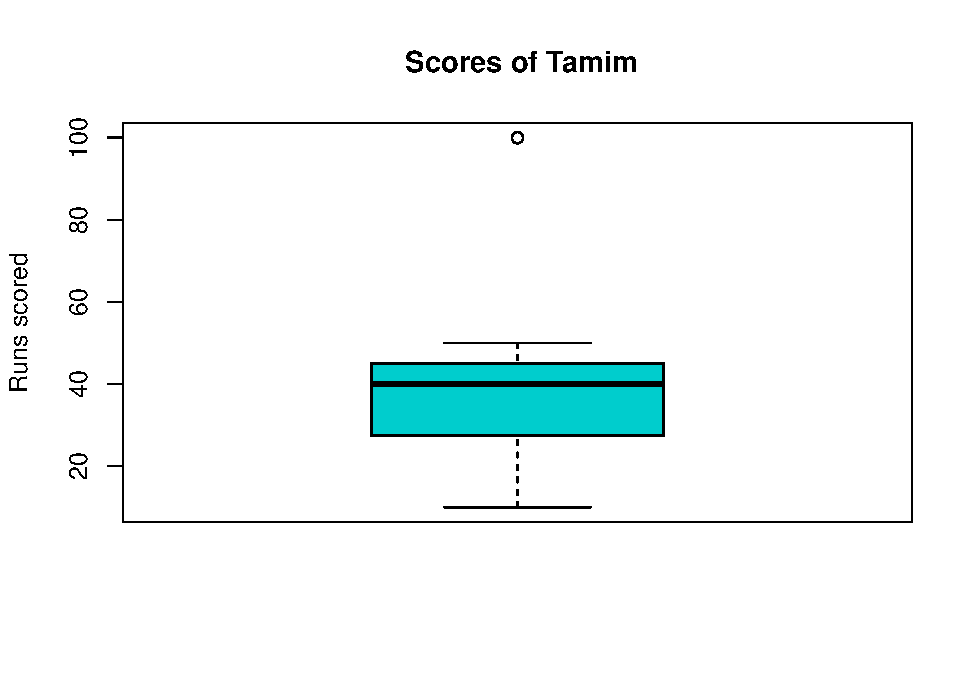
\includegraphics{Day_5_files/figure-latex/unnamed-chunk-4-1.pdf}

\begin{Shaded}
\begin{Highlighting}[]
\CommentTok{# Outlier is any value that is 1.5 times the IQR value above or }
\CommentTok{# below the Q3 or Q1 correspondingly. The score 100 is the outlier here.}

\KeywordTok{print}\NormalTok{(}\KeywordTok{paste}\NormalTok{(}\StringTok{"The outlier is:"}\NormalTok{, }\DecValTok{100}\NormalTok{))}
\end{Highlighting}
\end{Shaded}

\begin{verbatim}
## [1] "The outlier is: 100"
\end{verbatim}

\hypertarget{create-matrix-with-number-1-to-100.-the-matrix-should-contain-4-columns-and-25-rows.}{%
\section{4.Create matrix with number 1 to 100. The matrix should contain
4 columns and 25
rows.}\label{create-matrix-with-number-1-to-100.-the-matrix-should-contain-4-columns-and-25-rows.}}

\begin{Shaded}
\begin{Highlighting}[]
\NormalTok{mat <-}\StringTok{ }\KeywordTok{matrix}\NormalTok{(}\DecValTok{1}\OperatorTok{:}\DecValTok{100}\NormalTok{, }\DataTypeTok{nrow =} \DecValTok{25}\NormalTok{, }\DataTypeTok{ncol =} \DecValTok{4}\NormalTok{)}
\NormalTok{mat}
\end{Highlighting}
\end{Shaded}

\begin{verbatim}
##       [,1] [,2] [,3] [,4]
##  [1,]    1   26   51   76
##  [2,]    2   27   52   77
##  [3,]    3   28   53   78
##  [4,]    4   29   54   79
##  [5,]    5   30   55   80
##  [6,]    6   31   56   81
##  [7,]    7   32   57   82
##  [8,]    8   33   58   83
##  [9,]    9   34   59   84
## [10,]   10   35   60   85
## [11,]   11   36   61   86
## [12,]   12   37   62   87
## [13,]   13   38   63   88
## [14,]   14   39   64   89
## [15,]   15   40   65   90
## [16,]   16   41   66   91
## [17,]   17   42   67   92
## [18,]   18   43   68   93
## [19,]   19   44   69   94
## [20,]   20   45   70   95
## [21,]   21   46   71   96
## [22,]   22   47   72   97
## [23,]   23   48   73   98
## [24,]   24   49   74   99
## [25,]   25   50   75  100
\end{verbatim}

\hypertarget{give-the-4-column-names.-one-two-three-four.-it-should-look-like-following}{%
\section{5.Give the 4 column names. ``one, two, three, four''. It should
look like
following}\label{give-the-4-column-names.-one-two-three-four.-it-should-look-like-following}}

\begin{Shaded}
\begin{Highlighting}[]
\KeywordTok{colnames}\NormalTok{(mat) <-}\StringTok{ }\KeywordTok{c}\NormalTok{(}\StringTok{"one"}\NormalTok{, }\StringTok{"two"}\NormalTok{, }\StringTok{"three"}\NormalTok{, }\StringTok{"four"}\NormalTok{)}
\NormalTok{mat}
\end{Highlighting}
\end{Shaded}

\begin{verbatim}
##       one two three four
##  [1,]   1  26    51   76
##  [2,]   2  27    52   77
##  [3,]   3  28    53   78
##  [4,]   4  29    54   79
##  [5,]   5  30    55   80
##  [6,]   6  31    56   81
##  [7,]   7  32    57   82
##  [8,]   8  33    58   83
##  [9,]   9  34    59   84
## [10,]  10  35    60   85
## [11,]  11  36    61   86
## [12,]  12  37    62   87
## [13,]  13  38    63   88
## [14,]  14  39    64   89
## [15,]  15  40    65   90
## [16,]  16  41    66   91
## [17,]  17  42    67   92
## [18,]  18  43    68   93
## [19,]  19  44    69   94
## [20,]  20  45    70   95
## [21,]  21  46    71   96
## [22,]  22  47    72   97
## [23,]  23  48    73   98
## [24,]  24  49    74   99
## [25,]  25  50    75  100
\end{verbatim}

\begin{Shaded}
\begin{Highlighting}[]
\CommentTok{# Alternate approach}

\NormalTok{colname <-}\StringTok{ }\KeywordTok{c}\NormalTok{(}\StringTok{"one"}\NormalTok{, }\StringTok{"two"}\NormalTok{, }\StringTok{"three"}\NormalTok{, }\StringTok{"four"}\NormalTok{)}
\KeywordTok{colnames}\NormalTok{(mat) <-}\StringTok{ }\NormalTok{colname}
\NormalTok{mat}
\end{Highlighting}
\end{Shaded}

\begin{verbatim}
##       one two three four
##  [1,]   1  26    51   76
##  [2,]   2  27    52   77
##  [3,]   3  28    53   78
##  [4,]   4  29    54   79
##  [5,]   5  30    55   80
##  [6,]   6  31    56   81
##  [7,]   7  32    57   82
##  [8,]   8  33    58   83
##  [9,]   9  34    59   84
## [10,]  10  35    60   85
## [11,]  11  36    61   86
## [12,]  12  37    62   87
## [13,]  13  38    63   88
## [14,]  14  39    64   89
## [15,]  15  40    65   90
## [16,]  16  41    66   91
## [17,]  17  42    67   92
## [18,]  18  43    68   93
## [19,]  19  44    69   94
## [20,]  20  45    70   95
## [21,]  21  46    71   96
## [22,]  22  47    72   97
## [23,]  23  48    73   98
## [24,]  24  49    74   99
## [25,]  25  50    75  100
\end{verbatim}

\hypertarget{create-a-data-frame-that-looks-like-following.}{%
\section{6.Create a data frame that looks like
following.}\label{create-a-data-frame-that-looks-like-following.}}

\begin{Shaded}
\begin{Highlighting}[]
\NormalTok{Name <-}\StringTok{ }\KeywordTok{c}\NormalTok{(}\StringTok{"William"}\NormalTok{, }\StringTok{"Emma"}\NormalTok{, }\StringTok{"Sofia"}\NormalTok{, }\StringTok{"Markus"}\NormalTok{, }\StringTok{"Edward"}\NormalTok{, }\StringTok{"Thomas"}\NormalTok{)}
\NormalTok{Region <-}\StringTok{ }\KeywordTok{c}\NormalTok{(}\StringTok{"East"}\NormalTok{, }\StringTok{"North"}\NormalTok{, }\StringTok{"East"}\NormalTok{, }\StringTok{"South"}\NormalTok{, }\StringTok{"West"}\NormalTok{, }\StringTok{"West"}\NormalTok{)}
\NormalTok{Sales <-}\StringTok{ }\KeywordTok{c}\NormalTok{(}\DecValTok{50000}\NormalTok{, }\DecValTok{52000}\NormalTok{, }\DecValTok{90000}\NormalTok{, }\DecValTok{34000}\NormalTok{, }\DecValTok{42000}\NormalTok{, }\DecValTok{72000}\NormalTok{)}
\NormalTok{Expenses <-}\StringTok{ }\KeywordTok{c}\NormalTok{(}\DecValTok{42000}\NormalTok{, }\DecValTok{43000}\NormalTok{, }\DecValTok{50000}\NormalTok{, }\DecValTok{44000}\NormalTok{, }\DecValTok{38000}\NormalTok{, }\DecValTok{39000}\NormalTok{)}

\NormalTok{df <-}\StringTok{ }\KeywordTok{data.frame}\NormalTok{(Name, Region, Sales, Expenses)}
\NormalTok{df}
\end{Highlighting}
\end{Shaded}

\begin{verbatim}
##      Name Region Sales Expenses
## 1 William   East 50000    42000
## 2    Emma  North 52000    43000
## 3   Sofia   East 90000    50000
## 4  Markus  South 34000    44000
## 5  Edward   West 42000    38000
## 6  Thomas   West 72000    39000
\end{verbatim}

\hypertarget{create-the-following-list}{%
\section{7.Create the following list:}\label{create-the-following-list}}

\begin{Shaded}
\begin{Highlighting}[]
\NormalTok{mother <-}\StringTok{ "Veronique"}
\NormalTok{father <-}\StringTok{ "Michel"}
\NormalTok{sisters <-}\StringTok{ }\KeywordTok{c}\NormalTok{(}\StringTok{"Alicia"}\NormalTok{, }\StringTok{"Monica"}\NormalTok{)}
\NormalTok{sisters_age <-}\StringTok{ }\KeywordTok{c}\NormalTok{(}\DecValTok{12}\NormalTok{, }\DecValTok{22}\NormalTok{)}

\NormalTok{lst <-}\StringTok{ }\KeywordTok{list}\NormalTok{(mother, father, sisters, sisters_age)}
\NormalTok{lst}
\end{Highlighting}
\end{Shaded}

\begin{verbatim}
## [[1]]
## [1] "Veronique"
## 
## [[2]]
## [1] "Michel"
## 
## [[3]]
## [1] "Alicia" "Monica"
## 
## [[4]]
## [1] 12 22
\end{verbatim}

\begin{Shaded}
\begin{Highlighting}[]
\KeywordTok{names}\NormalTok{(lst) <-}\StringTok{ }\KeywordTok{c}\NormalTok{(}\StringTok{"mother"}\NormalTok{, }\StringTok{"father"}\NormalTok{, }\StringTok{"sisters"}\NormalTok{, }\StringTok{"sisters_age"}\NormalTok{)}
\NormalTok{lst}
\end{Highlighting}
\end{Shaded}

\begin{verbatim}
## $mother
## [1] "Veronique"
## 
## $father
## [1] "Michel"
## 
## $sisters
## [1] "Alicia" "Monica"
## 
## $sisters_age
## [1] 12 22
\end{verbatim}

\hypertarget{write-an-if-else-condition-where-it-says-if-x-is-greater-than-0-then-print-positive-if-less-than-0-print-negative-and-if-x-is-0-than-print-zero-and-if-anything-else-print-please-type-a-new-number.-check-what-the-value-shows-if-x---5-and-x---0}{%
\section{8.Write an if else condition where it says, if x is greater
than 0 then print positive, if less than 0 print negative and if x is 0
than print zero and if anything else print please type a new number.
Check what the value shows if x \textless{}- 5 and x \textless{}-
0}\label{write-an-if-else-condition-where-it-says-if-x-is-greater-than-0-then-print-positive-if-less-than-0-print-negative-and-if-x-is-0-than-print-zero-and-if-anything-else-print-please-type-a-new-number.-check-what-the-value-shows-if-x---5-and-x---0}}

\begin{Shaded}
\begin{Highlighting}[]
\NormalTok{x <-}\StringTok{ }\DecValTok{5}

\ControlFlowTok{if}\NormalTok{ (x }\OperatorTok{>}\StringTok{ }\DecValTok{0}\NormalTok{)\{}
  \KeywordTok{print}\NormalTok{(}\StringTok{"Positive"}\NormalTok{)}
\NormalTok{\} }\ControlFlowTok{else} \ControlFlowTok{if}\NormalTok{ (x }\OperatorTok{<}\StringTok{ }\DecValTok{0}\NormalTok{)\{}
  \KeywordTok{print}\NormalTok{(}\StringTok{"Negative"}\NormalTok{)}
\NormalTok{\} }\ControlFlowTok{else} \ControlFlowTok{if}\NormalTok{ (x }\OperatorTok{==}\StringTok{ }\DecValTok{0}\NormalTok{)\{}
  \KeywordTok{print}\NormalTok{(}\StringTok{"Zero"}\NormalTok{)}
\NormalTok{\} }\ControlFlowTok{else} 
  \KeywordTok{print}\NormalTok{(}\StringTok{"Please, type a new number"}\NormalTok{)}
\end{Highlighting}
\end{Shaded}

\begin{verbatim}
## [1] "Positive"
\end{verbatim}

\begin{Shaded}
\begin{Highlighting}[]
\NormalTok{x <-}\StringTok{ }\DecValTok{0}

\ControlFlowTok{if}\NormalTok{ (x }\OperatorTok{>}\StringTok{ }\DecValTok{0}\NormalTok{)\{}
  \KeywordTok{print}\NormalTok{(}\StringTok{"Positive"}\NormalTok{)}
\NormalTok{\} }\ControlFlowTok{else} \ControlFlowTok{if}\NormalTok{ (x }\OperatorTok{<}\StringTok{ }\DecValTok{0}\NormalTok{)\{}
  \KeywordTok{print}\NormalTok{(}\StringTok{"Negative"}\NormalTok{)}
\NormalTok{\} }\ControlFlowTok{else} \ControlFlowTok{if}\NormalTok{ (x }\OperatorTok{==}\StringTok{ }\DecValTok{0}\NormalTok{)\{}
  \KeywordTok{print}\NormalTok{(}\StringTok{"Zero"}\NormalTok{)}
\NormalTok{\} }\ControlFlowTok{else} 
  \KeywordTok{print}\NormalTok{(}\StringTok{"Please, type a new number"}\NormalTok{)}
\end{Highlighting}
\end{Shaded}

\begin{verbatim}
## [1] "Zero"
\end{verbatim}

\hypertarget{create-the-following-data-frame}{%
\section{9.Create the following data
frame:}\label{create-the-following-data-frame}}

\begin{Shaded}
\begin{Highlighting}[]
\NormalTok{DF1 <-}\StringTok{ }\KeywordTok{data.frame}\NormalTok{(}\DataTypeTok{c1 =} \KeywordTok{c}\NormalTok{(}\DecValTok{1}\NormalTok{,}\DecValTok{5}\NormalTok{,}\DecValTok{14}\NormalTok{,}\DecValTok{23}\NormalTok{,}\DecValTok{54}\NormalTok{), }
                  \DataTypeTok{c2 =} \KeywordTok{c}\NormalTok{(}\DecValTok{9}\NormalTok{,}\DecValTok{15}\NormalTok{,}\DecValTok{85}\NormalTok{,}\DecValTok{3}\NormalTok{,}\DecValTok{42}\NormalTok{), }
                  \DataTypeTok{c3 =} \KeywordTok{c}\NormalTok{(}\DecValTok{9}\NormalTok{,}\DecValTok{7}\NormalTok{,}\DecValTok{42}\NormalTok{,}\DecValTok{87}\NormalTok{,}\DecValTok{16}\NormalTok{))}
\NormalTok{DF1}
\end{Highlighting}
\end{Shaded}

\begin{verbatim}
##   c1 c2 c3
## 1  1  9  9
## 2  5 15  7
## 3 14 85 42
## 4 23  3 87
## 5 54 42 16
\end{verbatim}

\begin{Shaded}
\begin{Highlighting}[]
\NormalTok{mat1 <-}\StringTok{ }\KeywordTok{as.matrix}\NormalTok{(DF1)}
\NormalTok{mat1}
\end{Highlighting}
\end{Shaded}

\begin{verbatim}
##      c1 c2 c3
## [1,]  1  9  9
## [2,]  5 15  7
## [3,] 14 85 42
## [4,] 23  3 87
## [5,] 54 42 16
\end{verbatim}

\hypertarget{use-for-loop-to-get-the-following-output}{%
\section{10.Use for loop to get the following
output}\label{use-for-loop-to-get-the-following-output}}

\begin{Shaded}
\begin{Highlighting}[]
\NormalTok{digits <-}\StringTok{ }\KeywordTok{c}\NormalTok{(}\DecValTok{1}\OperatorTok{:}\DecValTok{10}\NormalTok{)}

\ControlFlowTok{for}\NormalTok{ (i }\ControlFlowTok{in}\NormalTok{ digits)\{}
  \KeywordTok{print}\NormalTok{(}\KeywordTok{paste}\NormalTok{(}\StringTok{"the year is,"}\NormalTok{, i))}
\NormalTok{\}}
\end{Highlighting}
\end{Shaded}

\begin{verbatim}
## [1] "the year is, 1"
## [1] "the year is, 2"
## [1] "the year is, 3"
## [1] "the year is, 4"
## [1] "the year is, 5"
## [1] "the year is, 6"
## [1] "the year is, 7"
## [1] "the year is, 8"
## [1] "the year is, 9"
## [1] "the year is, 10"
\end{verbatim}

\hypertarget{install-bioconductor-in-r.-install-deseq2-package-in-r.-check-the-following}{%
\section{11.Install Bioconductor in R. install Deseq2 package in R.
Check the
following}\label{install-bioconductor-in-r.-install-deseq2-package-in-r.-check-the-following}}

\url{https://www.bioconductor.org/packages/release/bioc/html/DESeq2.html}

\begin{Shaded}
\begin{Highlighting}[]
\CommentTok{# if (!requireNamespace("BiocManager", quietly = TRUE))}
\CommentTok{#    install.packages("BiocManager")}
\CommentTok{# BiocManager::install(version = "3.10")}

\CommentTok{# install Deseq2}
\CommentTok{# if (!requireNamespace("BiocManager", quietly = TRUE))}
\CommentTok{#    install.packages("BiocManager")}
\CommentTok{# BiocManager::install("DESeq2")}
\end{Highlighting}
\end{Shaded}

\hypertarget{load-the-inbuild-mtcars-data-frame-and-store-it-as-cars.-if-you-view-the-cars-you-can-see-that-the-first-column-is-mpg-and-fourth-column-is-hp.-swap-this-column-such-that-1st-column-is-hp-and-the-fourth-column-is-mpg.}{%
\section{12.Load the inbuild ``mtcars'' data frame and store it as
``cars''. If you View the cars you can see that the first column is
``mpg'' and fourth column is ``hp''. Swap this column such that 1st
column is ``hp'' and the fourth column is
``mpg''.}\label{load-the-inbuild-mtcars-data-frame-and-store-it-as-cars.-if-you-view-the-cars-you-can-see-that-the-first-column-is-mpg-and-fourth-column-is-hp.-swap-this-column-such-that-1st-column-is-hp-and-the-fourth-column-is-mpg.}}

\begin{Shaded}
\begin{Highlighting}[]
\KeywordTok{data}\NormalTok{(}\StringTok{"mtcars"}\NormalTok{)}
\NormalTok{cars <-}\StringTok{ }\NormalTok{mtcars}
\KeywordTok{str}\NormalTok{(cars)}
\end{Highlighting}
\end{Shaded}

\begin{verbatim}
## 'data.frame':    32 obs. of  11 variables:
##  $ mpg : num  21 21 22.8 21.4 18.7 18.1 14.3 24.4 22.8 19.2 ...
##  $ cyl : num  6 6 4 6 8 6 8 4 4 6 ...
##  $ disp: num  160 160 108 258 360 ...
##  $ hp  : num  110 110 93 110 175 105 245 62 95 123 ...
##  $ drat: num  3.9 3.9 3.85 3.08 3.15 2.76 3.21 3.69 3.92 3.92 ...
##  $ wt  : num  2.62 2.88 2.32 3.21 3.44 ...
##  $ qsec: num  16.5 17 18.6 19.4 17 ...
##  $ vs  : num  0 0 1 1 0 1 0 1 1 1 ...
##  $ am  : num  1 1 1 0 0 0 0 0 0 0 ...
##  $ gear: num  4 4 4 3 3 3 3 4 4 4 ...
##  $ carb: num  4 4 1 1 2 1 4 2 2 4 ...
\end{verbatim}

\begin{Shaded}
\begin{Highlighting}[]
\CommentTok{# View(cars)}

\KeywordTok{library}\NormalTok{(dplyr, }\DataTypeTok{quietly =} \OtherTok{TRUE}\NormalTok{)}
\end{Highlighting}
\end{Shaded}

\begin{verbatim}
## 
## Attaching package: 'dplyr'
\end{verbatim}

\begin{verbatim}
## The following objects are masked from 'package:stats':
## 
##     filter, lag
\end{verbatim}

\begin{verbatim}
## The following objects are masked from 'package:base':
## 
##     intersect, setdiff, setequal, union
\end{verbatim}

\begin{Shaded}
\begin{Highlighting}[]
\NormalTok{cars }\OperatorTok\StringTok{ }\KeywordTok{select}\NormalTok{(}\StringTok{"hp"}\NormalTok{, }\StringTok{"cyl"}\NormalTok{, }\StringTok{"disp"}\NormalTok{,}
                \StringTok{"mpg"}\NormalTok{, }\StringTok{"drat"}\NormalTok{, }\StringTok{"wt"}\NormalTok{, }
                \StringTok{"qsec"}\NormalTok{, }\StringTok{"vs"}\NormalTok{, }\StringTok{"am"}\NormalTok{, }
                \StringTok{"gear"}\NormalTok{, }\StringTok{"carb"}\NormalTok{)}
\end{Highlighting}
\end{Shaded}

\begin{verbatim}
##                      hp cyl  disp  mpg drat    wt  qsec vs am gear carb
## Mazda RX4           110   6 160.0 21.0 3.90 2.620 16.46  0  1    4    4
## Mazda RX4 Wag       110   6 160.0 21.0 3.90 2.875 17.02  0  1    4    4
## Datsun 710           93   4 108.0 22.8 3.85 2.320 18.61  1  1    4    1
## Hornet 4 Drive      110   6 258.0 21.4 3.08 3.215 19.44  1  0    3    1
## Hornet Sportabout   175   8 360.0 18.7 3.15 3.440 17.02  0  0    3    2
## Valiant             105   6 225.0 18.1 2.76 3.460 20.22  1  0    3    1
## Duster 360          245   8 360.0 14.3 3.21 3.570 15.84  0  0    3    4
## Merc 240D            62   4 146.7 24.4 3.69 3.190 20.00  1  0    4    2
## Merc 230             95   4 140.8 22.8 3.92 3.150 22.90  1  0    4    2
## Merc 280            123   6 167.6 19.2 3.92 3.440 18.30  1  0    4    4
## Merc 280C           123   6 167.6 17.8 3.92 3.440 18.90  1  0    4    4
## Merc 450SE          180   8 275.8 16.4 3.07 4.070 17.40  0  0    3    3
## Merc 450SL          180   8 275.8 17.3 3.07 3.730 17.60  0  0    3    3
## Merc 450SLC         180   8 275.8 15.2 3.07 3.780 18.00  0  0    3    3
## Cadillac Fleetwood  205   8 472.0 10.4 2.93 5.250 17.98  0  0    3    4
## Lincoln Continental 215   8 460.0 10.4 3.00 5.424 17.82  0  0    3    4
## Chrysler Imperial   230   8 440.0 14.7 3.23 5.345 17.42  0  0    3    4
## Fiat 128             66   4  78.7 32.4 4.08 2.200 19.47  1  1    4    1
## Honda Civic          52   4  75.7 30.4 4.93 1.615 18.52  1  1    4    2
## Toyota Corolla       65   4  71.1 33.9 4.22 1.835 19.90  1  1    4    1
## Toyota Corona        97   4 120.1 21.5 3.70 2.465 20.01  1  0    3    1
## Dodge Challenger    150   8 318.0 15.5 2.76 3.520 16.87  0  0    3    2
## AMC Javelin         150   8 304.0 15.2 3.15 3.435 17.30  0  0    3    2
## Camaro Z28          245   8 350.0 13.3 3.73 3.840 15.41  0  0    3    4
## Pontiac Firebird    175   8 400.0 19.2 3.08 3.845 17.05  0  0    3    2
## Fiat X1-9            66   4  79.0 27.3 4.08 1.935 18.90  1  1    4    1
## Porsche 914-2        91   4 120.3 26.0 4.43 2.140 16.70  0  1    5    2
## Lotus Europa        113   4  95.1 30.4 3.77 1.513 16.90  1  1    5    2
## Ford Pantera L      264   8 351.0 15.8 4.22 3.170 14.50  0  1    5    4
## Ferrari Dino        175   6 145.0 19.7 3.62 2.770 15.50  0  1    5    6
## Maserati Bora       335   8 301.0 15.0 3.54 3.570 14.60  0  1    5    8
## Volvo 142E          109   4 121.0 21.4 4.11 2.780 18.60  1  1    4    2
\end{verbatim}

\hypertarget{make-a-scatter-plot-mpg-vs-hp-and-color-it-based-on-gear.-what-is-the-difference-when-you-use-factor-and-when-you-dont}{%
\section{13.Make a scatter plot ``mpg'' vs ``hp'' and color it based on
``gear''. What is the difference when you use factor and when you
don't}\label{make-a-scatter-plot-mpg-vs-hp-and-color-it-based-on-gear.-what-is-the-difference-when-you-use-factor-and-when-you-dont}}

\begin{Shaded}
\begin{Highlighting}[]
\KeywordTok{library}\NormalTok{(ggplot2)}

\KeywordTok{head}\NormalTok{(cars)}
\end{Highlighting}
\end{Shaded}

\begin{verbatim}
##                    mpg cyl disp  hp drat    wt  qsec vs am gear carb
## Mazda RX4         21.0   6  160 110 3.90 2.620 16.46  0  1    4    4
## Mazda RX4 Wag     21.0   6  160 110 3.90 2.875 17.02  0  1    4    4
## Datsun 710        22.8   4  108  93 3.85 2.320 18.61  1  1    4    1
## Hornet 4 Drive    21.4   6  258 110 3.08 3.215 19.44  1  0    3    1
## Hornet Sportabout 18.7   8  360 175 3.15 3.440 17.02  0  0    3    2
## Valiant           18.1   6  225 105 2.76 3.460 20.22  1  0    3    1
\end{verbatim}

\begin{Shaded}
\begin{Highlighting}[]
\CommentTok{# Without factorization}
\KeywordTok{ggplot}\NormalTok{(}\DataTypeTok{data =}\NormalTok{ cars, }\KeywordTok{aes}\NormalTok{(}\DataTypeTok{x =}\NormalTok{ mpg , }\DataTypeTok{y =}\NormalTok{ hp, }\DataTypeTok{colour=}\NormalTok{ gear)) }\OperatorTok{+}\StringTok{ }
\StringTok{          }\KeywordTok{geom_point}\NormalTok{()}
\end{Highlighting}
\end{Shaded}

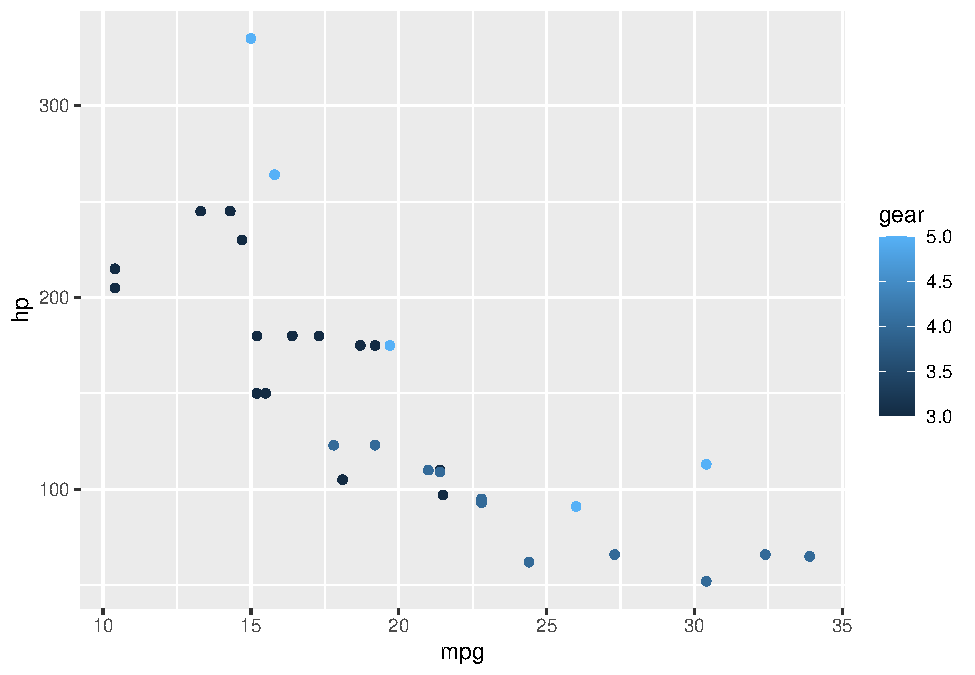
\includegraphics{Day_5_files/figure-latex/unnamed-chunk-14-1.pdf}

\begin{Shaded}
\begin{Highlighting}[]
\CommentTok{# With factorization}
\KeywordTok{ggplot}\NormalTok{(}\DataTypeTok{data =}\NormalTok{ cars, }\KeywordTok{aes}\NormalTok{(}\DataTypeTok{x =}\NormalTok{ mpg , }\DataTypeTok{y =}\NormalTok{ hp, }\DataTypeTok{colour=} \KeywordTok{factor}\NormalTok{(gear))) }\OperatorTok{+}\StringTok{ }
\StringTok{          }\KeywordTok{geom_point}\NormalTok{()}
\end{Highlighting}
\end{Shaded}

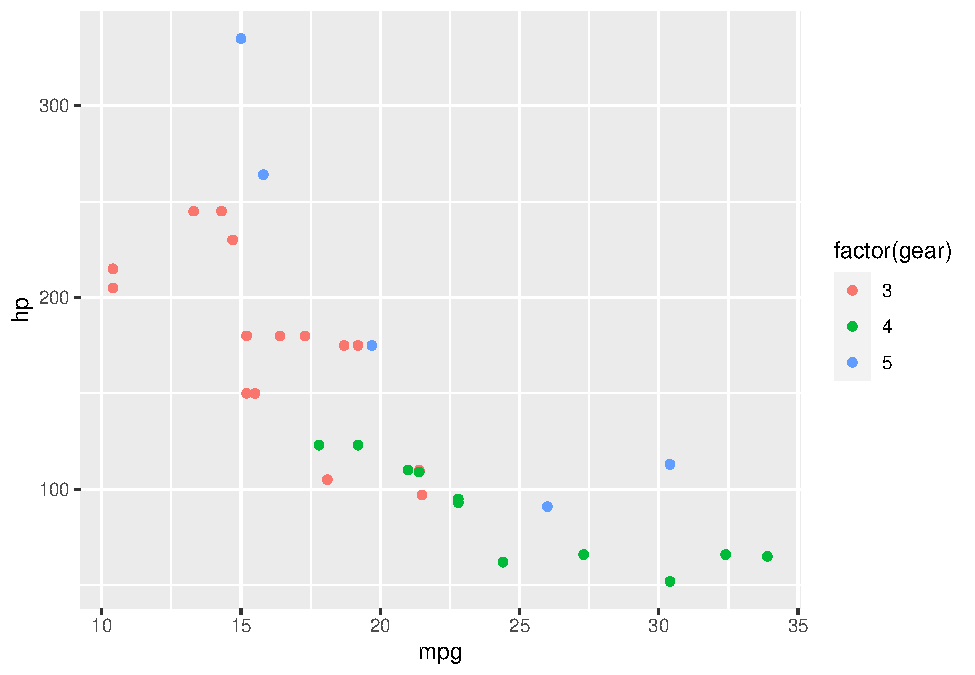
\includegraphics{Day_5_files/figure-latex/unnamed-chunk-14-2.pdf}

\begin{Shaded}
\begin{Highlighting}[]
\CommentTok{# We can make it more easy to understand using the shape argument}
\KeywordTok{ggplot}\NormalTok{(}\DataTypeTok{data =}\NormalTok{ cars, }\KeywordTok{aes}\NormalTok{(}\DataTypeTok{x =}\NormalTok{ mpg , }\DataTypeTok{y =}\NormalTok{ hp, }
                        \DataTypeTok{colour=} \KeywordTok{factor}\NormalTok{(gear), }
                        \DataTypeTok{shape =} \KeywordTok{factor}\NormalTok{(gear))) }\OperatorTok{+}\StringTok{ }
\StringTok{          }\KeywordTok{geom_point}\NormalTok{(}\DataTypeTok{size =} \FloatTok{1.5}\NormalTok{)}
\end{Highlighting}
\end{Shaded}

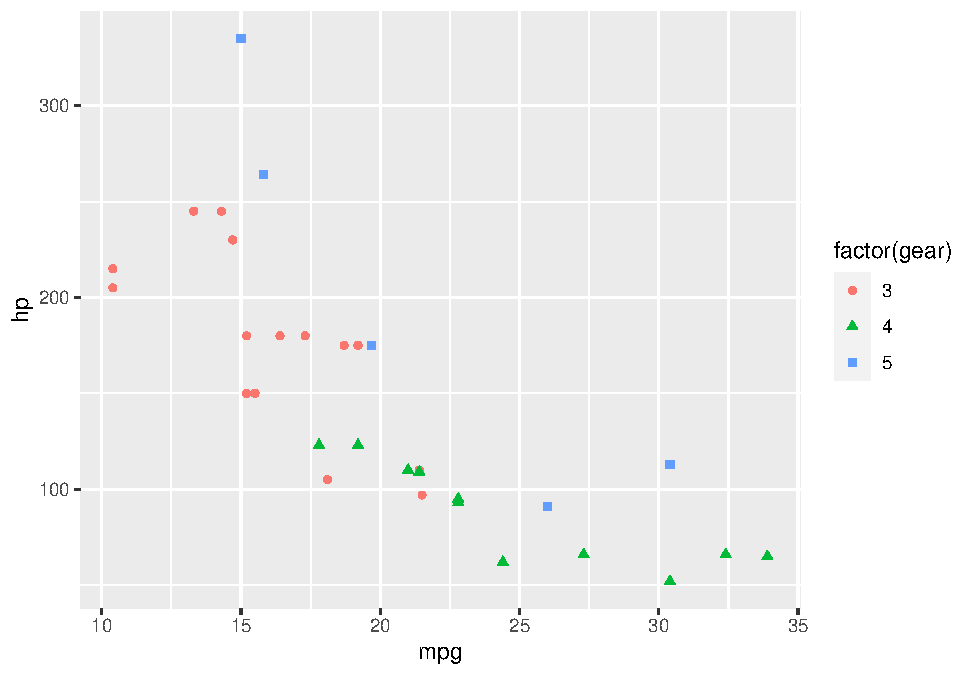
\includegraphics{Day_5_files/figure-latex/unnamed-chunk-14-3.pdf}

\hypertarget{load-the-file-house.csv-in-r.-you-can-see-that-the-aircond-column-has-0-or-1.-where-0-means-no-facility-of-air-condition-and-1-means-containing-facility-of-air-condition.}{%
\section{14.Load the file ``house.csv'' in R. you can see that the
``aircond'' column has 0 or 1. Where 0 means no facility of
air-condition and 1 means containing facility of
air-condition.}\label{load-the-file-house.csv-in-r.-you-can-see-that-the-aircond-column-has-0-or-1.-where-0-means-no-facility-of-air-condition-and-1-means-containing-facility-of-air-condition.}}

\begin{Shaded}
\begin{Highlighting}[]
\CommentTok{# Location of houses.csv file}

\NormalTok{data <-}\StringTok{ }\KeywordTok{read.csv}\NormalTok{(}\StringTok{"houses.csv"}\NormalTok{)}
\KeywordTok{str}\NormalTok{(data)}
\end{Highlighting}
\end{Shaded}

\begin{verbatim}
## 'data.frame':    1728 obs. of  16 variables:
##  $ X.1         : int  1 2 3 4 5 6 7 8 9 10 ...
##  $ X           : int  1 2 3 4 5 6 7 8 9 10 ...
##  $ price       : int  132500 181115 109000 155000 86060 120000 153000 170000 90000 122900 ...
##  $ lot_size    : num  0.09 0.92 0.19 0.41 0.11 0.68 0.4 1.21 0.83 1.94 ...
##  $ waterfront  : int  0 0 0 0 0 0 0 0 0 0 ...
##  $ age         : int  42 0 133 13 0 31 33 23 36 4 ...
##  $ land_value  : int  50000 22300 7300 18700 15000 14000 23300 14600 22200 21200 ...
##  $ construction: int  0 0 0 0 1 0 0 0 0 0 ...
##  $ air_cond    : int  0 0 0 0 1 0 0 0 0 0 ...
##  $ fuel        : int  3 2 2 2 2 2 4 4 3 2 ...
##  $ heat        : int  4 3 3 2 2 2 3 2 4 2 ...
##  $ sewer       : int  2 2 3 2 3 2 2 2 2 1 ...
##  $ living_area : int  906 1953 1944 1944 840 1152 2752 1662 1632 1416 ...
##  $ fireplaces  : int  1 0 1 1 0 1 1 1 0 0 ...
##  $ bathrooms   : num  1 2.5 1 1.5 1 1 1.5 1.5 1.5 1.5 ...
##  $ rooms       : int  5 6 8 5 3 8 8 9 8 6 ...
\end{verbatim}

\hypertarget{make-a-new-column-titled-new_created_column-which-contains-yes-or-no-value-which-is-consistent-with-0-and-1-in-aircond-column.}{%
\section{15.Make a new column titled ``New\_created\_column'' which
contains ``yes'' or ``no'' value which is consistent with 0 and 1 in
``aircond''
column.}\label{make-a-new-column-titled-new_created_column-which-contains-yes-or-no-value-which-is-consistent-with-0-and-1-in-aircond-column.}}

\begin{Shaded}
\begin{Highlighting}[]
\NormalTok{data <-}\StringTok{ }\NormalTok{data }\OperatorTok\StringTok{ }\KeywordTok{mutate}\NormalTok{( }\StringTok{"New_created_column"}\NormalTok{ =}\StringTok{ }
\StringTok{                           }\KeywordTok{ifelse}\NormalTok{(air_cond }\OperatorTok{==}\DecValTok{0}\NormalTok{, }\StringTok{"No"}\NormalTok{, }
                                  \KeywordTok{ifelse}\NormalTok{(air_cond }\OperatorTok{==}\StringTok{ }\DecValTok{1}\NormalTok{, }\StringTok{"Yes"}\NormalTok{, }\OtherTok{NA}\NormalTok{)))}

\KeywordTok{head}\NormalTok{(data }\OperatorTok\StringTok{ }\KeywordTok{select}\NormalTok{(air_cond, New_created_column))}
\end{Highlighting}
\end{Shaded}

\begin{verbatim}
##   air_cond New_created_column
## 1        0                 No
## 2        0                 No
## 3        0                 No
## 4        0                 No
## 5        1                Yes
## 6        0                 No
\end{verbatim}

\hypertarget{make-a-boxplot-with-x-axis-as-room-number-and-y-axis-as-price-and-compare-how-difference-in-price-it-makes-if-you-have-air-condition-facility-or-not.-use-new_created_column.}{%
\section{16.Make a boxplot with x axis as room number and y axis as
price and compare how difference in price it makes if you have air
condition facility or not. Use
new\_created\_column.}\label{make-a-boxplot-with-x-axis-as-room-number-and-y-axis-as-price-and-compare-how-difference-in-price-it-makes-if-you-have-air-condition-facility-or-not.-use-new_created_column.}}

\begin{Shaded}
\begin{Highlighting}[]
\KeywordTok{ggplot}\NormalTok{(}\DataTypeTok{data =}\NormalTok{ data, }\KeywordTok{aes}\NormalTok{(}\DataTypeTok{x =} \KeywordTok{factor}\NormalTok{(rooms), }
                        \DataTypeTok{y =}\NormalTok{ price, }
                        \DataTypeTok{colour =} \KeywordTok{factor}\NormalTok{(New_created_column))) }\OperatorTok{+}
\StringTok{  }\KeywordTok{geom_boxplot}\NormalTok{()}
\end{Highlighting}
\end{Shaded}

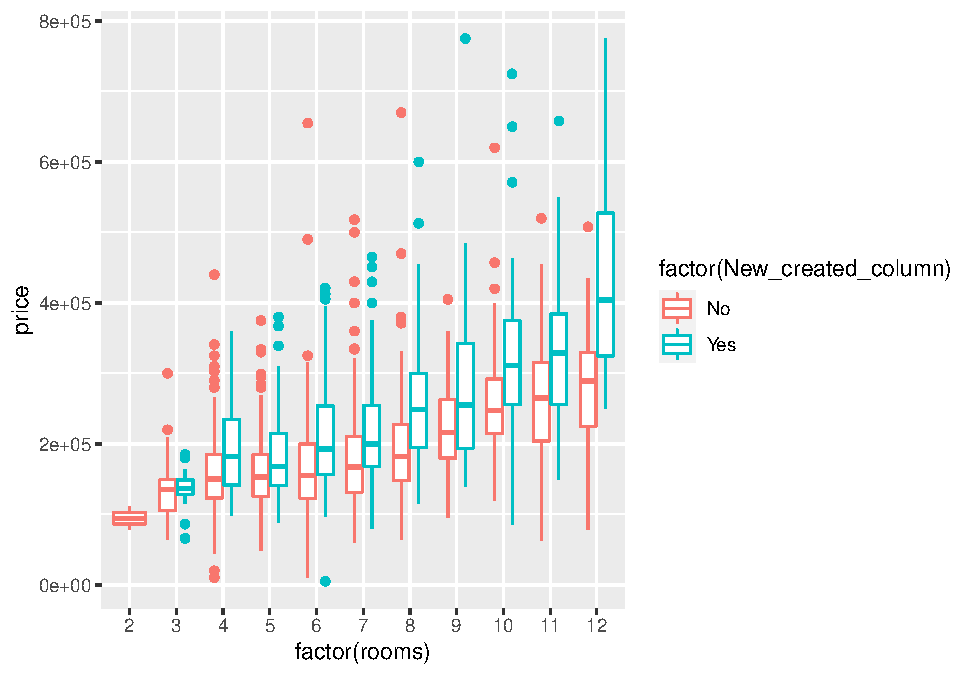
\includegraphics{Day_5_files/figure-latex/unnamed-chunk-17-1.pdf}

\hypertarget{create-a-frequency-polygon-with-facet_grid-based-on-new_created_column}{%
\section{17.Create a frequency polygon with facet\_grid based on
``New\_created\_column''}\label{create-a-frequency-polygon-with-facet_grid-based-on-new_created_column}}

\begin{Shaded}
\begin{Highlighting}[]
\KeywordTok{ggplot}\NormalTok{(}\DataTypeTok{data =}\NormalTok{ data, }\KeywordTok{aes}\NormalTok{(}\DataTypeTok{x =}\NormalTok{ price, }
                             \DataTypeTok{col =} \KeywordTok{factor}\NormalTok{(New_created_column)))}\OperatorTok{+}\StringTok{ }
\StringTok{  }\KeywordTok{geom_freqpoly}\NormalTok{(}\DataTypeTok{bins =} \DecValTok{100}\NormalTok{) }\OperatorTok{+}
\StringTok{  }\KeywordTok{facet_grid}\NormalTok{( }\OperatorTok{~}\StringTok{ }\NormalTok{New_created_column)}
\end{Highlighting}
\end{Shaded}

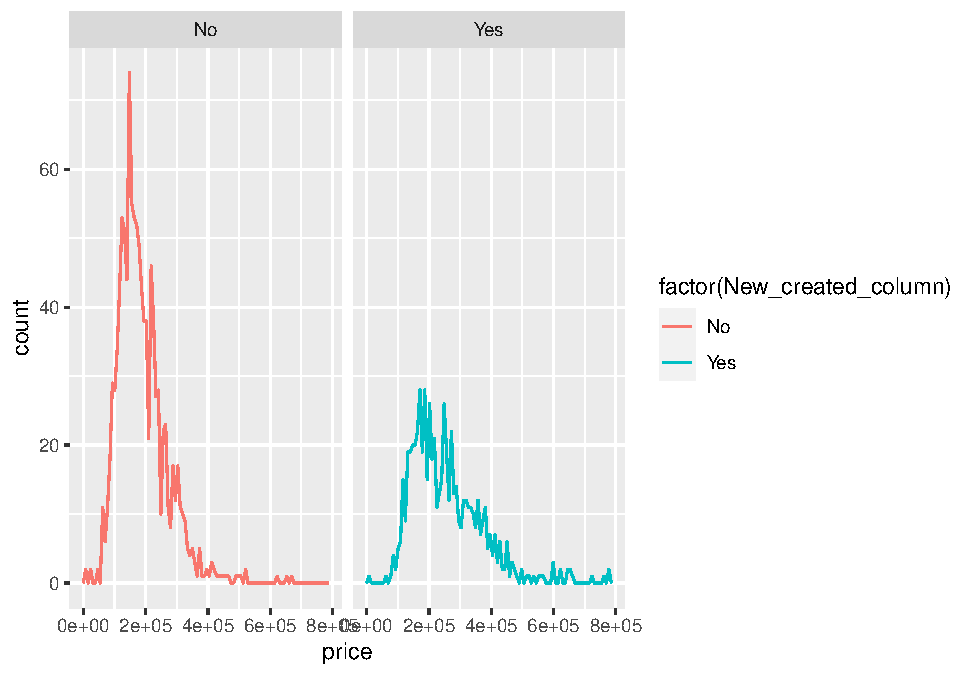
\includegraphics{Day_5_files/figure-latex/unnamed-chunk-18-1.pdf}

\hypertarget{say-you-have-three-genes-egfr-fox1-tf1.-you-have-calculated-that-in-three-cell-type-cell1-cell2-cell3.-you-want-to-create-a-matrix-where-each-gene-will-have-a-value-for-each-cell-type}{%
\section{18.Say you have three genes EGFR, FOX1, TF1. You have
calculated that in three cell type ``cell1, cell2, cell3''. You want to
create a matrix where each gene will have a value for each cell
type}\label{say-you-have-three-genes-egfr-fox1-tf1.-you-have-calculated-that-in-three-cell-type-cell1-cell2-cell3.-you-want-to-create-a-matrix-where-each-gene-will-have-a-value-for-each-cell-type}}

\begin{Shaded}
\begin{Highlighting}[]
\NormalTok{cell_}\DecValTok{1}\NormalTok{ <-}\StringTok{ }\KeywordTok{c}\NormalTok{(}\DecValTok{10}\NormalTok{, }\DecValTok{100}\NormalTok{, }\DecValTok{12}\NormalTok{)}
\NormalTok{cell_}\DecValTok{2}\NormalTok{ <-}\StringTok{ }\KeywordTok{c}\NormalTok{(}\DecValTok{12}\NormalTok{, }\DecValTok{12}\NormalTok{, }\DecValTok{2}\NormalTok{)}
\NormalTok{cell_}\DecValTok{3}\NormalTok{ <-}\StringTok{ }\KeywordTok{c}\NormalTok{(}\DecValTok{15}\NormalTok{, }\DecValTok{20}\NormalTok{, }\DecValTok{3}\NormalTok{)}

\NormalTok{data2 <-}\StringTok{ }\KeywordTok{data.frame}\NormalTok{(cell_}\DecValTok{1}\NormalTok{, cell_}\DecValTok{2}\NormalTok{, cell_}\DecValTok{3}\NormalTok{)}
\NormalTok{data2 <-}\StringTok{ }\KeywordTok{as.matrix}\NormalTok{(data2)}
\KeywordTok{rownames}\NormalTok{(data2) <-}\StringTok{ }\KeywordTok{c}\NormalTok{(}\StringTok{"EGFR"}\NormalTok{, }\StringTok{"TF_1"}\NormalTok{, }\StringTok{"FOX_1"}\NormalTok{)}
\NormalTok{data2}
\end{Highlighting}
\end{Shaded}

\begin{verbatim}
##       cell_1 cell_2 cell_3
## EGFR      10     12     15
## TF_1     100     12     20
## FOX_1     12      2      3
\end{verbatim}

\hypertarget{calculate-the-mean-of-each-row-and-add-it-as-the-fourth-column-and-calculate-the-row-sum-and-add-it-as-the-fifth-column}{%
\section{19.Calculate the mean of each row and add it as the fourth
column and calculate the row sum and add it as the fifth
column}\label{calculate-the-mean-of-each-row-and-add-it-as-the-fourth-column-and-calculate-the-row-sum-and-add-it-as-the-fifth-column}}

\begin{Shaded}
\begin{Highlighting}[]
\NormalTok{Mean <-}\StringTok{ }\KeywordTok{round}\NormalTok{(}\KeywordTok{rowMeans}\NormalTok{(data2),}\DecValTok{2}\NormalTok{)}

\NormalTok{Total <-}\StringTok{ }\KeywordTok{rowSums}\NormalTok{(data2)}

\KeywordTok{cbind}\NormalTok{(data2, Mean, Total)}
\end{Highlighting}
\end{Shaded}

\begin{verbatim}
##       cell_1 cell_2 cell_3  Mean Total
## EGFR      10     12     15 12.33    37
## TF_1     100     12     20 44.00   132
## FOX_1     12      2      3  5.67    17
\end{verbatim}

\hypertarget{say-you-have-collected-some-samples-from-5-person.-you-have-asked-them-if-they-believe-in-aliens.-the-response-was-as-follows}{%
\section{20.Say you have collected some samples from 5 person. You have
asked them if they believe in aliens. The response was as follows
:}\label{say-you-have-collected-some-samples-from-5-person.-you-have-asked-them-if-they-believe-in-aliens.-the-response-was-as-follows}}

\begin{Shaded}
\begin{Highlighting}[]
\NormalTok{responses <-}\StringTok{ }\KeywordTok{factor}\NormalTok{(}\KeywordTok{c}\NormalTok{(}\StringTok{"Agree"}\NormalTok{, }\StringTok{"Agree"}\NormalTok{, }\StringTok{"Strongly Agree"}\NormalTok{, }\StringTok{"Disagree"}\NormalTok{, }\StringTok{"Agree"}\NormalTok{))}

\KeywordTok{levels}\NormalTok{(responses) <-}\StringTok{ }\KeywordTok{c}\NormalTok{(}\StringTok{"Strongly Agree"}\NormalTok{,  }\StringTok{"Agree"}\NormalTok{, }\StringTok{"Disagree"}\NormalTok{)}
\NormalTok{responses}
\end{Highlighting}
\end{Shaded}

\begin{verbatim}
## [1] Strongly Agree Strongly Agree Disagree       Agree          Strongly Agree
## Levels: Strongly Agree Agree Disagree
\end{verbatim}

\hypertarget{create-the-following-data-frame-1}{%
\section{21.Create the following data
frame,}\label{create-the-following-data-frame-1}}

\begin{Shaded}
\begin{Highlighting}[]
\NormalTok{Age <-}\StringTok{ }\KeywordTok{as.numeric}\NormalTok{(}\KeywordTok{c}\NormalTok{(}\DecValTok{25}\NormalTok{, }\DecValTok{31}\NormalTok{, }\DecValTok{23}\NormalTok{, }\DecValTok{52}\NormalTok{, }\DecValTok{76}\NormalTok{, }\DecValTok{49}\NormalTok{, }\DecValTok{26}\NormalTok{))}
\NormalTok{Height <-}\StringTok{ }\KeywordTok{as.numeric}\NormalTok{(}\KeywordTok{c}\NormalTok{(}\DecValTok{177}\NormalTok{, }\DecValTok{163}\NormalTok{, }\DecValTok{190}\NormalTok{, }\DecValTok{179}\NormalTok{, }\DecValTok{163}\NormalTok{, }\DecValTok{183}\NormalTok{, }\DecValTok{164}\NormalTok{))}
\NormalTok{Weight <-}\StringTok{ }\KeywordTok{as.numeric}\NormalTok{(}\KeywordTok{c}\NormalTok{(}\DecValTok{57}\NormalTok{, }\DecValTok{69}\NormalTok{, }\DecValTok{83}\NormalTok{, }\DecValTok{75}\NormalTok{, }\DecValTok{70}\NormalTok{, }\DecValTok{83}\NormalTok{, }\DecValTok{53}\NormalTok{))}
\NormalTok{Sex <-}\StringTok{ }\KeywordTok{factor}\NormalTok{(}\KeywordTok{c}\NormalTok{(}\StringTok{"F"}\NormalTok{, }\StringTok{"F"}\NormalTok{, }\StringTok{"M"}\NormalTok{, }\StringTok{"M"}\NormalTok{, }\StringTok{"F"}\NormalTok{, }\StringTok{"M"}\NormalTok{, }\StringTok{"F"}\NormalTok{))}

\KeywordTok{levels}\NormalTok{(Sex) <-}\StringTok{ }\KeywordTok{c}\NormalTok{(}\StringTok{"F"}\NormalTok{, }\StringTok{"M"}\NormalTok{)}

\NormalTok{df <-}\StringTok{ }\KeywordTok{data.frame}\NormalTok{(Age, Height, Weight, Sex)}
\NormalTok{df}
\end{Highlighting}
\end{Shaded}

\begin{verbatim}
##   Age Height Weight Sex
## 1  25    177     57   F
## 2  31    163     69   F
## 3  23    190     83   M
## 4  52    179     75   M
## 5  76    163     70   F
## 6  49    183     83   M
## 7  26    164     53   F
\end{verbatim}

\begin{Shaded}
\begin{Highlighting}[]
\KeywordTok{rownames}\NormalTok{(df) <-}\StringTok{ }\KeywordTok{c}\NormalTok{(}\StringTok{"Alex"}\NormalTok{, }\StringTok{"Lilly"}\NormalTok{, }\StringTok{"Mark"}\NormalTok{, }\StringTok{"Oliver"}\NormalTok{, }\StringTok{"Martha"}\NormalTok{, }\StringTok{"Lucas"}\NormalTok{, }\StringTok{"Caroline"}\NormalTok{)}
\NormalTok{df}
\end{Highlighting}
\end{Shaded}

\begin{verbatim}
##          Age Height Weight Sex
## Alex      25    177     57   F
## Lilly     31    163     69   F
## Mark      23    190     83   M
## Oliver    52    179     75   M
## Martha    76    163     70   F
## Lucas     49    183     83   M
## Caroline  26    164     53   F
\end{verbatim}

\begin{Shaded}
\begin{Highlighting}[]
\NormalTok{df_recoded <-}\StringTok{ }\NormalTok{df }\OperatorTok\StringTok{ }\KeywordTok{mutate}\NormalTok{(}\DataTypeTok{Sex =} \KeywordTok{recode}\NormalTok{(Sex, }\StringTok{"F"}\NormalTok{ =}\StringTok{ "M"}\NormalTok{, }\StringTok{"M"}\NormalTok{ =}\StringTok{ "F"}\NormalTok{))}
\KeywordTok{rownames}\NormalTok{(df_recoded) <-}\StringTok{ }\KeywordTok{c}\NormalTok{(}\StringTok{"Alex"}\NormalTok{, }\StringTok{"Lilly"}\NormalTok{, }\StringTok{"Mark"}\NormalTok{, }
                          \StringTok{"Oliver"}\NormalTok{, }\StringTok{"Martha"}\NormalTok{, }\StringTok{"Lucas"}\NormalTok{, }\StringTok{"Caroline"}\NormalTok{)}
\NormalTok{df_recoded}
\end{Highlighting}
\end{Shaded}

\begin{verbatim}
##          Age Height Weight Sex
## Alex      25    177     57   M
## Lilly     31    163     69   M
## Mark      23    190     83   F
## Oliver    52    179     75   F
## Martha    76    163     70   M
## Lucas     49    183     83   F
## Caroline  26    164     53   M
\end{verbatim}

\hypertarget{create-this-data-frame-make-sure-you-import-the-variable-working-as-character-and-not-factor.}{%
\section{22.Create this data frame (make sure you import the variable
Working as character and not
factor).}\label{create-this-data-frame-make-sure-you-import-the-variable-working-as-character-and-not-factor.}}

\begin{Shaded}
\begin{Highlighting}[]
\NormalTok{Working <-}\StringTok{ }\KeywordTok{c}\NormalTok{(}\StringTok{"Yes"}\NormalTok{, }\StringTok{"No"}\NormalTok{, }\StringTok{"No"}\NormalTok{, }\StringTok{"Yes"}\NormalTok{, }\StringTok{"Yes"}\NormalTok{, }\StringTok{"No"}\NormalTok{, }\StringTok{"Yes"}\NormalTok{)}
\KeywordTok{class}\NormalTok{(Working)}
\end{Highlighting}
\end{Shaded}

\begin{verbatim}
## [1] "character"
\end{verbatim}

\begin{Shaded}
\begin{Highlighting}[]
\NormalTok{df_working <-}\StringTok{ }\KeywordTok{data.frame}\NormalTok{(Working, }\DataTypeTok{stringsAsFactors =}\NormalTok{ F)}
\KeywordTok{rownames}\NormalTok{(df_working) <-}\StringTok{ }\KeywordTok{c}\NormalTok{(}\StringTok{"Alex"}\NormalTok{, }\StringTok{"Lilly"}\NormalTok{, }\StringTok{"Mark"}\NormalTok{, }\StringTok{"Oliver"}\NormalTok{, }\StringTok{"Martha"}\NormalTok{, }\StringTok{"Lucas"}\NormalTok{, }\StringTok{"Caroline"}\NormalTok{)}


\NormalTok{df_new <-}\StringTok{ }\KeywordTok{cbind}\NormalTok{(df, df_working)}
\NormalTok{df_new}
\end{Highlighting}
\end{Shaded}

\begin{verbatim}
##          Age Height Weight Sex Working
## Alex      25    177     57   F     Yes
## Lilly     31    163     69   F      No
## Mark      23    190     83   M      No
## Oliver    52    179     75   M     Yes
## Martha    76    163     70   F     Yes
## Lucas     49    183     83   M      No
## Caroline  26    164     53   F     Yes
\end{verbatim}

\begin{Shaded}
\begin{Highlighting}[]
\NormalTok{nr <-}\StringTok{ }\KeywordTok{nrow}\NormalTok{(df_new)}
\NormalTok{nc <-}\StringTok{ }\KeywordTok{ncol}\NormalTok{(df_new)}

\KeywordTok{print}\NormalTok{(}\KeywordTok{paste}\NormalTok{(}\StringTok{"Rows:"}\NormalTok{, nr, }\StringTok{"Columns:"}\NormalTok{, nc))}
\end{Highlighting}
\end{Shaded}

\begin{verbatim}
## [1] "Rows: 7 Columns: 5"
\end{verbatim}

\begin{Shaded}
\begin{Highlighting}[]
\KeywordTok{lapply}\NormalTok{(df_new, class)}
\end{Highlighting}
\end{Shaded}

\begin{verbatim}
## $Age
## [1] "numeric"
## 
## $Height
## [1] "numeric"
## 
## $Weight
## [1] "numeric"
## 
## $Sex
## [1] "factor"
## 
## $Working
## [1] "character"
\end{verbatim}

\hypertarget{write-two-string-hello-and-why-am-i-doing-this.-add-this-two-string-together-and-separate-by}{%
\section{23.Write two string ``hello'' and ``why am I doing this''. Add
this two string together and separate by
``,''}\label{write-two-string-hello-and-why-am-i-doing-this.-add-this-two-string-together-and-separate-by}}

\begin{Shaded}
\begin{Highlighting}[]
\NormalTok{string1 <-}\StringTok{ "Hello"}
\NormalTok{string2 <-}\StringTok{ "why am I doing this"}
\NormalTok{str3 <-}\StringTok{ "because Sohan vai told me to do so !!"}

\KeywordTok{print}\NormalTok{(}\KeywordTok{paste}\NormalTok{(string1, string2, str3, }\DataTypeTok{sep =} \StringTok{", "}\NormalTok{))}
\end{Highlighting}
\end{Shaded}

\begin{verbatim}
## [1] "Hello, why am I doing this, because Sohan vai told me to do so !!"
\end{verbatim}

\hypertarget{if-name_list---lista-1200-b-this-is-a-string-c-hello.-you-will-write-a-code-that-will-add-1-to-each-element-of-the-first-vector-of-the-new-list.-also-add-a-new-item-z-newitem-to-the-list-name_list}{%
\section{24.If name\_list \textless{}- list(a = 1:200, b = ``this is a
string'', c = ``hello''). You will write a code that will add 1 to each
element of the first vector of the new list. Also, add a new item z =
``newItem'' to the list
name\_list}\label{if-name_list---lista-1200-b-this-is-a-string-c-hello.-you-will-write-a-code-that-will-add-1-to-each-element-of-the-first-vector-of-the-new-list.-also-add-a-new-item-z-newitem-to-the-list-name_list}}

\begin{Shaded}
\begin{Highlighting}[]
\NormalTok{name_list <-}\StringTok{ }\KeywordTok{list}\NormalTok{(}\DataTypeTok{a =} \DecValTok{1}\OperatorTok{:}\DecValTok{200}\NormalTok{, }\DataTypeTok{b =} \StringTok{"this is a string"}\NormalTok{, }\DataTypeTok{c =} \StringTok{"hello"}\NormalTok{)}
\NormalTok{name_list}
\end{Highlighting}
\end{Shaded}

\begin{verbatim}
## $a
##   [1]   1   2   3   4   5   6   7   8   9  10  11  12  13  14  15  16  17  18
##  [19]  19  20  21  22  23  24  25  26  27  28  29  30  31  32  33  34  35  36
##  [37]  37  38  39  40  41  42  43  44  45  46  47  48  49  50  51  52  53  54
##  [55]  55  56  57  58  59  60  61  62  63  64  65  66  67  68  69  70  71  72
##  [73]  73  74  75  76  77  78  79  80  81  82  83  84  85  86  87  88  89  90
##  [91]  91  92  93  94  95  96  97  98  99 100 101 102 103 104 105 106 107 108
## [109] 109 110 111 112 113 114 115 116 117 118 119 120 121 122 123 124 125 126
## [127] 127 128 129 130 131 132 133 134 135 136 137 138 139 140 141 142 143 144
## [145] 145 146 147 148 149 150 151 152 153 154 155 156 157 158 159 160 161 162
## [163] 163 164 165 166 167 168 169 170 171 172 173 174 175 176 177 178 179 180
## [181] 181 182 183 184 185 186 187 188 189 190 191 192 193 194 195 196 197 198
## [199] 199 200
## 
## $b
## [1] "this is a string"
## 
## $c
## [1] "hello"
\end{verbatim}

\begin{Shaded}
\begin{Highlighting}[]
\NormalTok{name_list[[}\StringTok{"a"}\NormalTok{]]}
\end{Highlighting}
\end{Shaded}

\begin{verbatim}
##   [1]   1   2   3   4   5   6   7   8   9  10  11  12  13  14  15  16  17  18
##  [19]  19  20  21  22  23  24  25  26  27  28  29  30  31  32  33  34  35  36
##  [37]  37  38  39  40  41  42  43  44  45  46  47  48  49  50  51  52  53  54
##  [55]  55  56  57  58  59  60  61  62  63  64  65  66  67  68  69  70  71  72
##  [73]  73  74  75  76  77  78  79  80  81  82  83  84  85  86  87  88  89  90
##  [91]  91  92  93  94  95  96  97  98  99 100 101 102 103 104 105 106 107 108
## [109] 109 110 111 112 113 114 115 116 117 118 119 120 121 122 123 124 125 126
## [127] 127 128 129 130 131 132 133 134 135 136 137 138 139 140 141 142 143 144
## [145] 145 146 147 148 149 150 151 152 153 154 155 156 157 158 159 160 161 162
## [163] 163 164 165 166 167 168 169 170 171 172 173 174 175 176 177 178 179 180
## [181] 181 182 183 184 185 186 187 188 189 190 191 192 193 194 195 196 197 198
## [199] 199 200
\end{verbatim}

\begin{Shaded}
\begin{Highlighting}[]
\NormalTok{add_vector <-}\StringTok{ }\KeywordTok{rep.int}\NormalTok{(}\DataTypeTok{x =} \DecValTok{1}\NormalTok{, }\DecValTok{200}\NormalTok{)}
\NormalTok{add_vector}
\end{Highlighting}
\end{Shaded}

\begin{verbatim}
##   [1] 1 1 1 1 1 1 1 1 1 1 1 1 1 1 1 1 1 1 1 1 1 1 1 1 1 1 1 1 1 1 1 1 1 1 1 1 1
##  [38] 1 1 1 1 1 1 1 1 1 1 1 1 1 1 1 1 1 1 1 1 1 1 1 1 1 1 1 1 1 1 1 1 1 1 1 1 1
##  [75] 1 1 1 1 1 1 1 1 1 1 1 1 1 1 1 1 1 1 1 1 1 1 1 1 1 1 1 1 1 1 1 1 1 1 1 1 1
## [112] 1 1 1 1 1 1 1 1 1 1 1 1 1 1 1 1 1 1 1 1 1 1 1 1 1 1 1 1 1 1 1 1 1 1 1 1 1
## [149] 1 1 1 1 1 1 1 1 1 1 1 1 1 1 1 1 1 1 1 1 1 1 1 1 1 1 1 1 1 1 1 1 1 1 1 1 1
## [186] 1 1 1 1 1 1 1 1 1 1 1 1 1 1 1
\end{verbatim}

\begin{Shaded}
\begin{Highlighting}[]
\NormalTok{a <-}\StringTok{ }\NormalTok{name_list[[}\StringTok{"a"}\NormalTok{]] }\OperatorTok{+}\StringTok{ }\NormalTok{add_vector}
\NormalTok{a}
\end{Highlighting}
\end{Shaded}

\begin{verbatim}
##   [1]   2   3   4   5   6   7   8   9  10  11  12  13  14  15  16  17  18  19
##  [19]  20  21  22  23  24  25  26  27  28  29  30  31  32  33  34  35  36  37
##  [37]  38  39  40  41  42  43  44  45  46  47  48  49  50  51  52  53  54  55
##  [55]  56  57  58  59  60  61  62  63  64  65  66  67  68  69  70  71  72  73
##  [73]  74  75  76  77  78  79  80  81  82  83  84  85  86  87  88  89  90  91
##  [91]  92  93  94  95  96  97  98  99 100 101 102 103 104 105 106 107 108 109
## [109] 110 111 112 113 114 115 116 117 118 119 120 121 122 123 124 125 126 127
## [127] 128 129 130 131 132 133 134 135 136 137 138 139 140 141 142 143 144 145
## [145] 146 147 148 149 150 151 152 153 154 155 156 157 158 159 160 161 162 163
## [163] 164 165 166 167 168 169 170 171 172 173 174 175 176 177 178 179 180 181
## [181] 182 183 184 185 186 187 188 189 190 191 192 193 194 195 196 197 198 199
## [199] 200 201
\end{verbatim}

\begin{Shaded}
\begin{Highlighting}[]
\NormalTok{name_list <-}\StringTok{ }\KeywordTok{list}\NormalTok{(}\DataTypeTok{a =}\NormalTok{ a, }\DataTypeTok{b =} \StringTok{"this is a string"}\NormalTok{, }
                  \DataTypeTok{c =} \StringTok{"hello"}\NormalTok{, }\DataTypeTok{z =} \StringTok{"newItem"}\NormalTok{)}
\NormalTok{name_list}
\end{Highlighting}
\end{Shaded}

\begin{verbatim}
## $a
##   [1]   2   3   4   5   6   7   8   9  10  11  12  13  14  15  16  17  18  19
##  [19]  20  21  22  23  24  25  26  27  28  29  30  31  32  33  34  35  36  37
##  [37]  38  39  40  41  42  43  44  45  46  47  48  49  50  51  52  53  54  55
##  [55]  56  57  58  59  60  61  62  63  64  65  66  67  68  69  70  71  72  73
##  [73]  74  75  76  77  78  79  80  81  82  83  84  85  86  87  88  89  90  91
##  [91]  92  93  94  95  96  97  98  99 100 101 102 103 104 105 106 107 108 109
## [109] 110 111 112 113 114 115 116 117 118 119 120 121 122 123 124 125 126 127
## [127] 128 129 130 131 132 133 134 135 136 137 138 139 140 141 142 143 144 145
## [145] 146 147 148 149 150 151 152 153 154 155 156 157 158 159 160 161 162 163
## [163] 164 165 166 167 168 169 170 171 172 173 174 175 176 177 178 179 180 181
## [181] 182 183 184 185 186 187 188 189 190 191 192 193 194 195 196 197 198 199
## [199] 200 201
## 
## $b
## [1] "this is a string"
## 
## $c
## [1] "hello"
## 
## $z
## [1] "newItem"
\end{verbatim}

\hypertarget{download-the-small_counts.txt-from-the-following-location}{%
\section{25.Download the small\_counts.txt from the following
location}\label{download-the-small_counts.txt-from-the-following-location}}

\begin{Shaded}
\begin{Highlighting}[]
\CommentTok{# file <- "https://figshare.com/s/1d788fd384d33e913a2a"}
\CommentTok{# dest <- paste(getwd(), "small_counts.txt", sep = "/")}
\CommentTok{# dest}

\CommentTok{# if (file.exists(dest) == !T) \{}
\CommentTok{#  download.file(file, dest, method = "wget", mode = "w")}
\CommentTok{# \} else \{}
\CommentTok{#  print("File is already downloaded !")}
\CommentTok{# \}}

\CommentTok{### This is a link to the folder. We can download it manually }
\CommentTok{## by going to the browser and opening the folder and downloading }
\CommentTok{## the file manually.}

\CommentTok{### Or we can download the file from R by the direct link to the file.}
\StringTok{"https://ndownloader.figshare.com/files/6005547?private_link=1d788fd384d33e913a2a"}
\end{Highlighting}
\end{Shaded}

\begin{verbatim}
## [1] "https://ndownloader.figshare.com/files/6005547?private_link=1d788fd384d33e913a2a"
\end{verbatim}

\begin{Shaded}
\begin{Highlighting}[]
\NormalTok{file <-}\StringTok{ "https://ndownloader.figshare.com/files/6005547?private_link=1d788fd384d33e913a2a"}
\NormalTok{dest <-}\StringTok{ }\KeywordTok{paste}\NormalTok{(}\KeywordTok{getwd}\NormalTok{(), }\StringTok{"small_counts.txt"}\NormalTok{, }\DataTypeTok{sep =} \StringTok{"/"}\NormalTok{)}
\NormalTok{dest}
\end{Highlighting}
\end{Shaded}

\begin{verbatim}
## [1] "/Users/marufahmedbhuiyan/Desktop/cBALST_R/Day 5- 10 July 2020/small_counts.txt"
\end{verbatim}

\begin{Shaded}
\begin{Highlighting}[]
\ControlFlowTok{if}\NormalTok{ (}\KeywordTok{file.exists}\NormalTok{(dest) }\OperatorTok{==}\StringTok{ }\OperatorTok{!}\NormalTok{T) \{}
  \KeywordTok{download.file}\NormalTok{(file, dest, }\DataTypeTok{method =} \StringTok{"auto"}\NormalTok{)}
\NormalTok{\} }\ControlFlowTok{else}\NormalTok{ \{}
  \KeywordTok{print}\NormalTok{(}\StringTok{"File is already downloaded !"}\NormalTok{)}
\NormalTok{\}}
\end{Highlighting}
\end{Shaded}

\begin{verbatim}
## [1] "File is already downloaded !"
\end{verbatim}

\hypertarget{read-the-file-in-r-and-save-it-as-small_counts.-view-the-file.}{%
\section{26.Read the file in R and save it as small\_counts. View the
file.}\label{read-the-file-in-r-and-save-it-as-small_counts.-view-the-file.}}

\begin{Shaded}
\begin{Highlighting}[]
\NormalTok{small_counts <-}\StringTok{ }\KeywordTok{read.table}\NormalTok{(}\StringTok{"small_counts.txt"}\NormalTok{, }\DataTypeTok{header =} \OtherTok{TRUE}\NormalTok{)}
\NormalTok{small_counts}
\end{Highlighting}
\end{Shaded}

\begin{verbatim}
##         Sample_1 Sample_2 Sample_3 Sample_4
## Xkr4         438      300       65      237
## Sox17        106      182       82      105
## Mrpl15       309      234      337      300
## Lypla1       652      515      948      935
## Tcea1       1604     1495     1721     1317
## Rgs20          4        2       14        4
## Atp6v1h      769      752     1062      987
## Rb1cc1      1494     1412     1157      967
## Pcmtd1      1344     1242     1374     1593
## Rrs1        1691     1808     2127     1653
\end{verbatim}

\begin{Shaded}
\begin{Highlighting}[]
\CommentTok{#View(small_counts)}
\end{Highlighting}
\end{Shaded}

\hypertarget{get-the-following-output-from-the-file}{%
\section{27.Get the following output from the
file}\label{get-the-following-output-from-the-file}}

\begin{Shaded}
\begin{Highlighting}[]
\NormalTok{small_counts[,}\DecValTok{1}\OperatorTok{:}\DecValTok{2}\NormalTok{]}
\end{Highlighting}
\end{Shaded}

\begin{verbatim}
##         Sample_1 Sample_2
## Xkr4         438      300
## Sox17        106      182
## Mrpl15       309      234
## Lypla1       652      515
## Tcea1       1604     1495
## Rgs20          4        2
## Atp6v1h      769      752
## Rb1cc1      1494     1412
## Pcmtd1      1344     1242
## Rrs1        1691     1808
\end{verbatim}

\hypertarget{get-log-of-the-small_count-so-that-it-looks-like-the-following}{%
\section{28.Get log of the small\_count so that it looks like the
following}\label{get-log-of-the-small_count-so-that-it-looks-like-the-following}}

\begin{Shaded}
\begin{Highlighting}[]
\KeywordTok{log}\NormalTok{(small_counts)}
\end{Highlighting}
\end{Shaded}

\begin{verbatim}
##         Sample_1  Sample_2 Sample_3 Sample_4
## Xkr4    6.082219 5.7037825 4.174387 5.468060
## Sox17   4.663439 5.2040067 4.406719 4.653960
## Mrpl15  5.733341 5.4553211 5.820083 5.703782
## Lypla1  6.480045 6.2441669 6.854355 6.840547
## Tcea1   7.380256 7.3098815 7.450661 7.183112
## Rgs20   1.386294 0.6931472 2.639057 1.386294
## Atp6v1h 6.645091 6.6227363 6.967909 6.894670
## Rb1cc1  7.309212 7.2527624 7.053586 6.874198
## Pcmtd1  7.203406 7.1244783 7.225481 7.373374
## Rrs1    7.433075 7.4999765 7.662468 7.410347
\end{verbatim}

\hypertarget{download-the-resultstable_small.txt-from-the-following-location-httpsfigshare.coms1d788fd384d33e913a2a}{%
\section{\texorpdfstring{29.Download the ``ResultsTable\_small.txt''
from the following location
``\url{https://figshare.com/s/1d788fd384d33e913a2a}''}{29.Download the ``ResultsTable\_small.txt'' from the following location ``https://figshare.com/s/1d788fd384d33e913a2a''}}\label{download-the-resultstable_small.txt-from-the-following-location-httpsfigshare.coms1d788fd384d33e913a2a}}

\begin{Shaded}
\begin{Highlighting}[]
\CommentTok{### This is a link to the folder. We can download it manually }
\CommentTok{### by going to the browser and opening the folder and }
\CommentTok{### downloading the file manually.}

\CommentTok{### Or we can download the file from R by the direct link to the file.}
\CommentTok{# "https://ndownloader.figshare.com/files/6005550?private_link=1d788fd384d33e913a2a"}

\NormalTok{file <-}\StringTok{ }
\StringTok{  "https://ndownloader.figshare.com/files/6005550?private_link=1d788fd384d33e913a2a"}
\NormalTok{dest <-}\StringTok{ }\KeywordTok{paste}\NormalTok{(}\KeywordTok{getwd}\NormalTok{(), }\StringTok{"ResultsTable_small.txt"}\NormalTok{, }\DataTypeTok{sep =} \StringTok{"/"}\NormalTok{)}
\NormalTok{dest}
\end{Highlighting}
\end{Shaded}

\begin{verbatim}
## [1] "/Users/marufahmedbhuiyan/Desktop/cBALST_R/Day 5- 10 July 2020/ResultsTable_small.txt"
\end{verbatim}

\begin{Shaded}
\begin{Highlighting}[]
\ControlFlowTok{if}\NormalTok{ (}\KeywordTok{file.exists}\NormalTok{(dest) }\OperatorTok{==}\StringTok{ }\OperatorTok{!}\NormalTok{T) \{}
  \KeywordTok{download.file}\NormalTok{(file, dest, }\DataTypeTok{method =} \StringTok{"auto"}\NormalTok{)}
\NormalTok{\} }\ControlFlowTok{else}\NormalTok{ \{}
  \KeywordTok{print}\NormalTok{(}\StringTok{"File is already downloaded !"}\NormalTok{)}
\NormalTok{\}}
\end{Highlighting}
\end{Shaded}

\begin{verbatim}
## [1] "File is already downloaded !"
\end{verbatim}

\hypertarget{this-is-a-file-which-contains-the-gene-expression-data.-the-entrez-id-is-the-gene-name.-you-can-search-entrez-id-in-google-to-get-more-information.symbol-is-the-gene-name.-and-logfc-value-which-means-how-much-more-a-gene-is-expressed-in-treatment-condition-compared-to-control-condition.-read-the-file-in-r-and-store-it-as-results.}{%
\section{30.This is a file which contains the gene expression data. The
Entrez id is the gene name. You can search Entrez id in google to get
more information.Symbol is the gene name. And ``logFC'' value which
means how much more a gene is expressed in treatment condition compared
to control condition. Read the file in R and store it as
``results''.}\label{this-is-a-file-which-contains-the-gene-expression-data.-the-entrez-id-is-the-gene-name.-you-can-search-entrez-id-in-google-to-get-more-information.symbol-is-the-gene-name.-and-logfc-value-which-means-how-much-more-a-gene-is-expressed-in-treatment-condition-compared-to-control-condition.-read-the-file-in-r-and-store-it-as-results.}}

\begin{Shaded}
\begin{Highlighting}[]
\NormalTok{results <-}\StringTok{ }\KeywordTok{read.table}\NormalTok{(dest, }\DataTypeTok{header =}\NormalTok{ T)}
\KeywordTok{head}\NormalTok{(results)}
\end{Highlighting}
\end{Shaded}

\begin{verbatim}
##   ENTREZID        SYMBOL     logFC  AveExpr         t      P.Value   adj.P.Val
## 1    24117          Wif1  1.819943 2.975545  20.10780 1.063770e-10 1.01624e-06
## 2   381290        Atp2b4 -2.143885 3.944066 -19.07495 1.982934e-10 1.01624e-06
## 3    78896 1500015O10Rik  2.807548 3.036519  18.54773 2.758828e-10 1.01624e-06
## 4   226101          Myof -2.329744 6.223525 -18.26861 3.297667e-10 1.01624e-06
## 5    16012        Igfbp6 -2.896115 1.978449 -18.21525 3.413066e-10 1.01624e-06
## 6   231830       Micall2  2.253400 4.760597  18.02627 3.858161e-10 1.01624e-06
\end{verbatim}

\begin{Shaded}
\begin{Highlighting}[]
\KeywordTok{str}\NormalTok{(results)}
\end{Highlighting}
\end{Shaded}

\begin{verbatim}
## 'data.frame':    40 obs. of  7 variables:
##  $ ENTREZID : int  24117 381290 78896 226101 16012 231830 16669 55987 231991 14620 ...
##  $ SYMBOL   : Factor w/ 40 levels "1500015O10Rik",..: 40 3 1 26 20 23 21 8 9 16 ...
##  $ logFC    : num  1.82 -2.14 2.81 -2.33 -2.9 ...
##  $ AveExpr  : num  2.98 3.94 3.04 6.22 1.98 ...
##  $ t        : num  20.1 -19.1 18.5 -18.3 -18.2 ...
##  $ P.Value  : num  1.06e-10 1.98e-10 2.76e-10 3.30e-10 3.41e-10 ...
##  $ adj.P.Val: num  1.02e-06 1.02e-06 1.02e-06 1.02e-06 1.02e-06 ...
\end{verbatim}

\hypertarget{sort-the-file-such-thath-the-genes-are-orderd-in-highest-to-lowest-value-of-logfc.}{%
\section{31.Sort the file such thath the genes are orderd in highest to
lowest value of
``logFC''.}\label{sort-the-file-such-thath-the-genes-are-orderd-in-highest-to-lowest-value-of-logfc.}}

\begin{Shaded}
\begin{Highlighting}[]
\KeywordTok{head}\NormalTok{(results[,}\DecValTok{1}\OperatorTok{:}\DecValTok{3}\NormalTok{], }\DecValTok{10}\NormalTok{)}
\end{Highlighting}
\end{Shaded}

\begin{verbatim}
##    ENTREZID        SYMBOL     logFC
## 1     24117          Wif1  1.819943
## 2    381290        Atp2b4 -2.143885
## 3     78896 1500015O10Rik  2.807548
## 4    226101          Myof -2.329744
## 5     16012        Igfbp6 -2.896115
## 6    231830       Micall2  2.253400
## 7     16669         Krt19 -2.312721
## 8     55987         Cpxm2 -1.515469
## 9    231991         Creb5 -2.598105
## 10    14620          Gjb3  3.600094
\end{verbatim}

\begin{Shaded}
\begin{Highlighting}[]
\KeywordTok{head}\NormalTok{(results[}\KeywordTok{order}\NormalTok{(}\OperatorTok{-}\NormalTok{results}\OperatorTok{$}\NormalTok{logFC),],}\DecValTok{10}\NormalTok{)}
\end{Highlighting}
\end{Shaded}

\begin{verbatim}
##    ENTREZID        SYMBOL    logFC  AveExpr        t      P.Value    adj.P.Val
## 22    16878           Lif 3.738933 6.682034 13.73344 9.105708e-09 6.541210e-06
## 10    14620          Gjb3 3.600094 3.525281 16.46627 1.113755e-09 1.718703e-06
## 25    12977          Csf1 2.835624 7.477591 13.41902 1.187300e-08 7.505634e-06
## 3     78896 1500015O10Rik 2.807548 3.036519 18.54773 2.758828e-10 1.016240e-06
## 15    11636           Ak1 2.766745 4.303475 15.27694 2.664640e-09 2.807465e-06
## 26    12654         Chil1 2.342914 5.576457 13.21976 1.408760e-08 8.306595e-06
## 29   217166         Nr1d1 2.278879 6.260878 13.12885 1.524242e-08 8.306595e-06
## 6    231830       Micall2 2.253400 4.760597 18.02627 3.858161e-10 1.016240e-06
## 13    74747         Ddit4 2.180370 6.864791 15.70145 1.938279e-09 2.356351e-06
## 20    17131         Smad7 1.972771 6.717519 14.14348 6.493642e-09 5.131276e-06
\end{verbatim}

\hypertarget{see-the-following-figure}{%
\section{32.See the following figure}\label{see-the-following-figure}}

Type the above code in your console and check counts\_matrix to see what
does it create. What do you think ``rpois'' comment did here? And try to
find what is the difference between paste and paste0. Always remember
``google'' is your friend.

\begin{Shaded}
\begin{Highlighting}[]
\NormalTok{counts_matrix <-}\StringTok{ }\KeywordTok{data.frame}\NormalTok{(}\DataTypeTok{cell_1 =} \KeywordTok{rpois}\NormalTok{(}\DecValTok{10}\NormalTok{,}\DecValTok{10}\NormalTok{),}
                            \DataTypeTok{cell_2 =} \KeywordTok{rpois}\NormalTok{(}\DecValTok{10}\NormalTok{,}\DecValTok{10}\NormalTok{),}
                            \DataTypeTok{cell_3 =} \KeywordTok{rpois}\NormalTok{(}\DecValTok{10}\NormalTok{, }\DecValTok{30}\NormalTok{))}
\KeywordTok{rownames}\NormalTok{(counts_matrix) <-}\StringTok{ }\KeywordTok{paste0}\NormalTok{(}\StringTok{"gene_"}\NormalTok{, }\DecValTok{1}\OperatorTok{:}\DecValTok{10}\NormalTok{)}
\NormalTok{counts_matrix <-}\StringTok{ }\KeywordTok{as.matrix}\NormalTok{(counts_matrix)}
\NormalTok{counts_matrix}
\end{Highlighting}
\end{Shaded}

\begin{verbatim}
##         cell_1 cell_2 cell_3
## gene_1       9     12     28
## gene_2      12     10     36
## gene_3       9     11     38
## gene_4      10      8     35
## gene_5      17     12     32
## gene_6       3     15     28
## gene_7      10      8     38
## gene_8      11      7     23
## gene_9       9     10     28
## gene_10     10     13     32
\end{verbatim}

\begin{Shaded}
\begin{Highlighting}[]
\CommentTok{## What do you think “rpois” comment did here? }
\CommentTok{## And try to find what is the difference between paste and paste0.}

\CommentTok{## rpois generates a Poisson distribution with random deviates. }
\CommentTok{## Other similar terms are dpois (density), qpois(quantile), }
\CommentTok{## ppois (log distribution function)}

\CommentTok{## The Poisson distribution is the discrete probability}
\CommentTok{## distribution of the number of events occurring in a }
\CommentTok{## given time period, given the average number of times }
\CommentTok{## the event occurs over that time period.}

\CommentTok{## The difference between paste() and paste0() is that }
\CommentTok{## the argument sep by default is " " (paste) and "" }
\CommentTok{## (paste0). paste0() is faster than paste() if our }
\CommentTok{## objective is concatenate strings without spaces }
\CommentTok{## because we don’t have to  specify the argument sep. }
\CommentTok{## For example...see the difference between these..}

\KeywordTok{paste0}\NormalTok{(}\StringTok{"gene_"}\NormalTok{, }\DecValTok{1}\OperatorTok{:}\DecValTok{10}\NormalTok{)}
\end{Highlighting}
\end{Shaded}

\begin{verbatim}
##  [1] "gene_1"  "gene_2"  "gene_3"  "gene_4"  "gene_5"  "gene_6"  "gene_7" 
##  [8] "gene_8"  "gene_9"  "gene_10"
\end{verbatim}

\begin{Shaded}
\begin{Highlighting}[]
\KeywordTok{paste}\NormalTok{(}\StringTok{"gene_"}\NormalTok{, }\DecValTok{1}\OperatorTok{:}\DecValTok{10}\NormalTok{)}
\end{Highlighting}
\end{Shaded}

\begin{verbatim}
##  [1] "gene_ 1"  "gene_ 2"  "gene_ 3"  "gene_ 4"  "gene_ 5"  "gene_ 6" 
##  [7] "gene_ 7"  "gene_ 8"  "gene_ 9"  "gene_ 10"
\end{verbatim}

\hypertarget{create-a-heatmap-from-the-using-the-following-file-explain-what-was-done-in-each-line.-use-to-comment-on-your-code-file-in-r}{%
\section{33.Create a heatmap from the using the following file: Explain
what was done in each line. Use ``\#\#'' to comment on your code file in
R}\label{create-a-heatmap-from-the-using-the-following-file-explain-what-was-done-in-each-line.-use-to-comment-on-your-code-file-in-r}}

Load the file ``basketball.csv''. Make sure you change the read.csv
location from the following code.

The code will/might show you error!.copy the error and put it in google
and see what is the suggestion from the internet. Try to understand and
solve the problem. The end of the code will show something like the
following:

\begin{Shaded}
\begin{Highlighting}[]
\KeywordTok{file.exists}\NormalTok{(}\StringTok{"basketball.csv"}\NormalTok{)}
\end{Highlighting}
\end{Shaded}

\begin{verbatim}
## [1] TRUE
\end{verbatim}

\begin{Shaded}
\begin{Highlighting}[]
\CommentTok{# importing the file}
\NormalTok{nba <-}\StringTok{ }\KeywordTok{read.csv}\NormalTok{(}\StringTok{"basketball.csv"}\NormalTok{)}

\CommentTok{# sorting the file accoring to PTS in increasing order}
\NormalTok{nba <-}\StringTok{ }\NormalTok{nba[}\KeywordTok{order}\NormalTok{(nba}\OperatorTok{$}\NormalTok{PTS),]}

\CommentTok{# Naming the rownames according to the Name column}
\KeywordTok{row.names}\NormalTok{(nba) <-}\StringTok{ }\NormalTok{nba}\OperatorTok{$}\NormalTok{Name}

\CommentTok{# Subsetting the data frame with all rows and }
\CommentTok{# 20 columns except the first one}
\NormalTok{nba <-}\StringTok{ }\NormalTok{nba[,}\DecValTok{2}\OperatorTok{:}\DecValTok{20}\NormalTok{]}

\CommentTok{# Creating a matrix}
\NormalTok{nba_matrix <-}\StringTok{ }\KeywordTok{data.matrix}\NormalTok{(nba)}

\CommentTok{# Creating a heatmap}
\NormalTok{nba_heatmap <-}\StringTok{ }\KeywordTok{heatmap}\NormalTok{(nba_matrix, }\DataTypeTok{Rowv =} \OtherTok{NA}\NormalTok{, }
                       \DataTypeTok{Colv =} \OtherTok{NA}\NormalTok{, }
                       \DataTypeTok{col =} \KeywordTok{cm.colors}\NormalTok{(}\DecValTok{256}\NormalTok{),}
                       \DataTypeTok{scale =} \StringTok{"column"}\NormalTok{,}
                       \DataTypeTok{margins =} \KeywordTok{c}\NormalTok{(}\DecValTok{5}\NormalTok{,}\DecValTok{10}\NormalTok{))}
\end{Highlighting}
\end{Shaded}

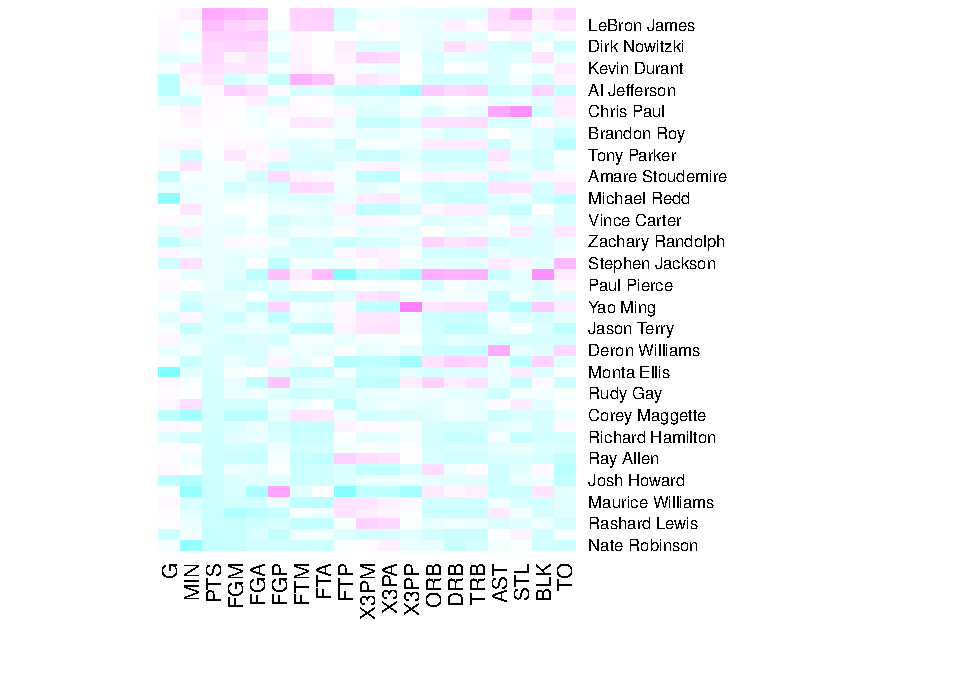
\includegraphics{Day_5_files/figure-latex/unnamed-chunk-34-1.pdf}

\begin{Shaded}
\begin{Highlighting}[]
\CommentTok{# The code didn't show any error to me ! So, let's continue}

\CommentTok{# I prefer the following color scheme better}
\NormalTok{nba_heatmap <-}\StringTok{ }\KeywordTok{heatmap}\NormalTok{(nba_matrix, }\DataTypeTok{Rowv =} \OtherTok{NA}\NormalTok{, }
                       \DataTypeTok{Colv =} \OtherTok{NA}\NormalTok{, }
                       \DataTypeTok{col =} \KeywordTok{heat.colors}\NormalTok{(}\DecValTok{256}\NormalTok{),}
                       \DataTypeTok{scale =} \StringTok{"column"}\NormalTok{,}
                       \DataTypeTok{margins =} \KeywordTok{c}\NormalTok{(}\DecValTok{5}\NormalTok{,}\DecValTok{10}\NormalTok{))}
\end{Highlighting}
\end{Shaded}

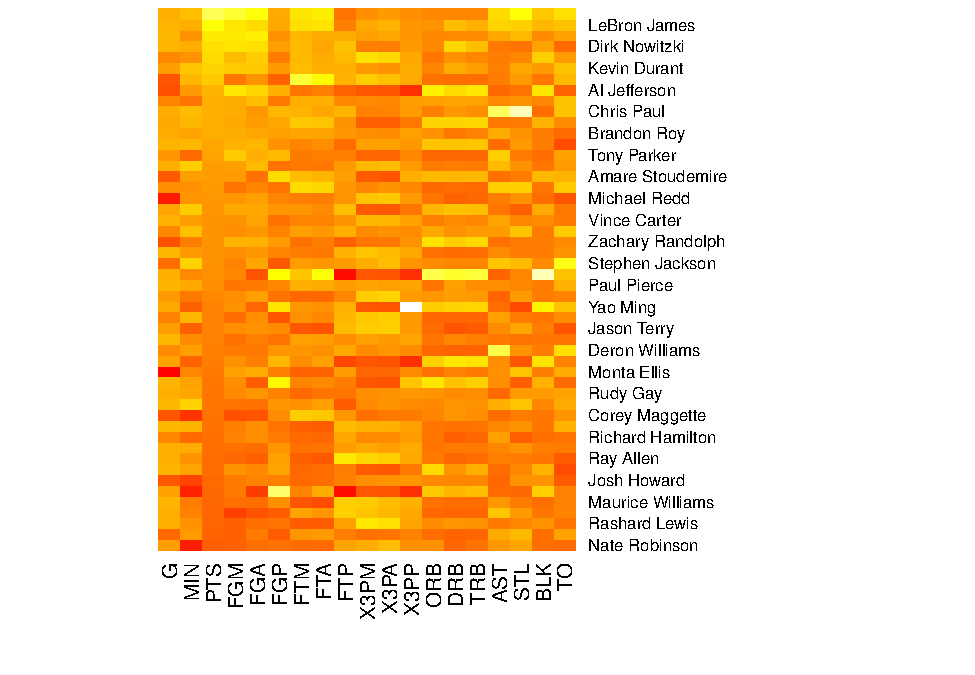
\includegraphics{Day_5_files/figure-latex/unnamed-chunk-34-2.pdf}

\begin{Shaded}
\begin{Highlighting}[]
\CommentTok{# Blue is my favorite color. So, let's color it blue !!}
\ControlFlowTok{if}\NormalTok{ (}\OperatorTok{!}\KeywordTok{require}\NormalTok{(}\StringTok{"RColorBrewer"}\NormalTok{)) \{}
\KeywordTok{install.packages}\NormalTok{(}\StringTok{"RColorBrewer"}\NormalTok{)}
\KeywordTok{library}\NormalTok{(RColorBrewer)}
\NormalTok{\}}
\end{Highlighting}
\end{Shaded}

\begin{verbatim}
## Loading required package: RColorBrewer
\end{verbatim}

\begin{Shaded}
\begin{Highlighting}[]
\NormalTok{nba_heatmap <-}\StringTok{ }\KeywordTok{heatmap}\NormalTok{(nba_matrix, }\DataTypeTok{Rowv =} \OtherTok{NA}\NormalTok{, }
                       \DataTypeTok{Colv =} \OtherTok{NA}\NormalTok{, }
                       \DataTypeTok{col =} \KeywordTok{brewer.pal}\NormalTok{(}\DecValTok{9}\NormalTok{, }\StringTok{"Blues"}\NormalTok{),}
                       \DataTypeTok{scale =} \StringTok{"column"}\NormalTok{,}
                       \DataTypeTok{margins =} \KeywordTok{c}\NormalTok{(}\DecValTok{5}\NormalTok{,}\DecValTok{10}\NormalTok{))}
\end{Highlighting}
\end{Shaded}

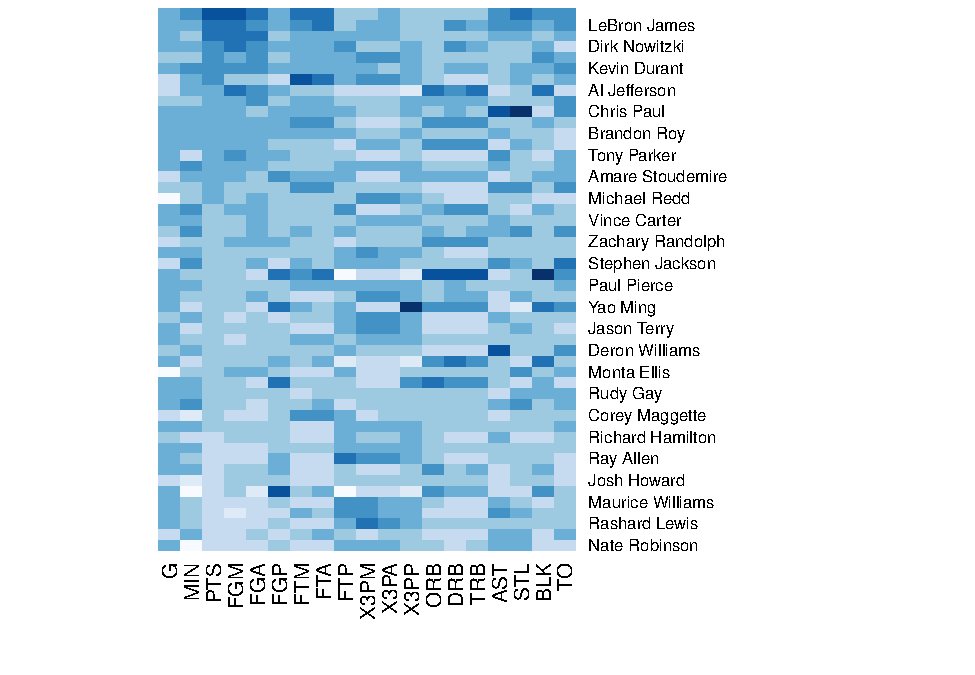
\includegraphics{Day_5_files/figure-latex/unnamed-chunk-34-3.pdf}

\end{document}
